% Chapter 5

\chapter{Event Identity Information Management (EIIM) Life Cycle for Social Media} % Main chapter title

\label{eiim} % For referencing the chapter elsewhere, use \ref{Chapter1} 

\lhead{Chapter 5. \emph{Event Identity Information Management (EIIM) Life Cycle for Social Media}} % This is for the header on each page - perhaps a shortened title


%\section{Background : Entity Identity Information Management}

This chapter discusses about the Event Identity Information Management framework in order to solve the problems posed in Chapter \ref{events}, Section \ref{problem}

\begin{figure}[htbp]
  \caption{Identity Integrity component of the EIIM life cycle.}
  \centering
    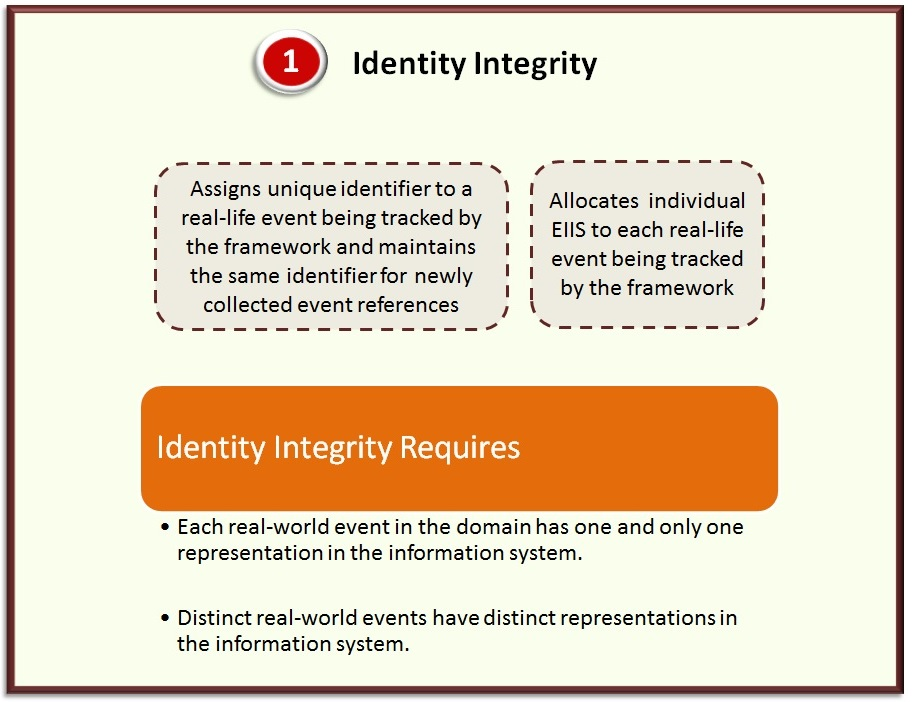
\includegraphics[width=14cm,height=11cm]{Figures/EIIMComponents/IdentityIntegrity.jpg}
\end{figure}

\section{Identity Integrity}
One of the fundamental goals of the proposed framework is to maintain a one-to-one correspondence between real-world events being monitored and the Event Identity Information Structure (EIIS) of the corresponding events for ensuring identity integrity. Therefore, a separate EIIS is maintained corresponding to each event. As new events are introduced to the framework, a unique identifier is assigned to them along with the allocation of individual EIIS structures. The framework is expected to maintain the integrity throughout the EIIM life cycle, by consistently assigning the same identifier to the references of a tracked event. Modules of this component assigns 12 byte unique integers known as ObjectId  to each event, and is also responsible for maintaining the same ObjectId for event ids of collected references and related EIIS. It is also the functionality of this component to assign the right identifier to the references resolved for an event by the Event Reference Resolution component.


\section{Event Reference Collection\label{eventreferencecollection}}

\begin{figure}[htbp]
  \caption{Event Reference Collection component of the EIIM life cycle.}
  \centering
    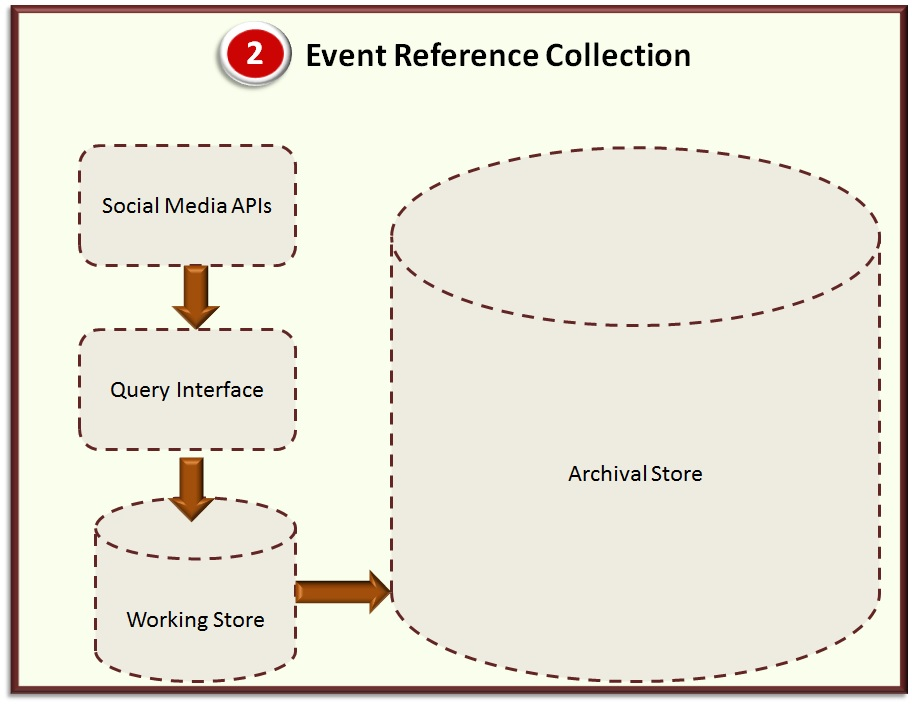
\includegraphics[width=14cm,height=11cm]{Figures/EIIMComponents/EventReferenceCollection.jpg}
\end{figure}

This component allows the framework to collect event references from different social media websites using its publicly available APIs (Application Programming Interface), and store them in the database after processing them using the next two components of the EIIM life cycle. Due to the semi-structured nature of the collected data, a NOSQL document oriented database management system (MongoDb ) is used for storage. The choice of MongoDb was also driven by its ability to scale horizontally and perform operations on large volumes of data. A query interface is implemented that allows an user of the system to pass query parameters (for example event related hashtags and key words) that bootstraps the data collection and event tracking process. As already shown in Table \ref{socialmediametadata} most of the popular social media channels allow hashtags, the data for the experiments were collected using a popular hashtag for the respective events. 

%For performing the experiments, data was collected from two types of social media websites, 
%\begin{itemize}
%\item \textbf{Blogs} - representing the longer genre of textual references.
%\item \textbf{Microblogs} - representing the shorter genre of textual references.
%\end{itemize}

%The query interface for blogs was implemented separately from the other social media channels as blogs don't provide any API for collecting data. Either one has to scrap data from search engines or monitor the RSS feeds of a pre-specified list of blogs. Details of the data collected is presented next. 

%\noindent \textbf{\textit{Motivation behind source selection:}} For many people blogs have become popular social media sources for satisfying interpersonal communication needs. Blogs act as a platform for masses to share their likes and dislikes, voice their opinions, provide suggestions and report news. Over the years blogging has matured from personal diaries to citizen journalistic sources providing live coverage of events beyond the professional newsrooms. Often mainstream media rely on blogs for reporting first-hand accounts of an event \cite{ekdale2007expression}. Other social media platforms like microblogs, social networks etc., also promote such activities. But, these platforms have very little scope to elaborately discuss about the events due to the limitations in the length of content allowed to be posted. However, these alternative platforms act as good sources for studying and tracking dissemination of information during real-life events. This motivated us to perform our experiments on sources collected from the blogging platforms instead of other social media webs

Due to extreme popularity of Twitter, data from it was collected for representing the microblog genre and short textual social media references. Four million tweets (approx) related to five different events were collected. Details of the collected event references are provided in Table \ref{informationcuedata}. The tweets were collected over the given period of time, by providing a popular hashtag to the Twitter streaming API  as shown in Table \ref{informationcuedata} (for details about Twitter Data Collection please refer Appendix \ref{AppendixA}). Only English language tweets are considered for the experiments as the available natural language toolkits performs well for English, and the annotators used for different tasks are only proficient in English language.

\begin{table}[htbp]
\center
\caption{Details of data collected for analyzing event related tweet content.}
\label{informationcuedata}
\begin{tabular}{|c|c|c|c|}
\hline
\textbf{Event} & \textbf{Query Hashtag}                          & \shortstack{\textbf{No. of} \\ \textbf{Tweets}} & \shortstack{\textbf{Time Period}}                               \\ \hline
\shortstack{Sochi Winter\\ Games 2014 \\ ($http://goo.gl/sG4Rqd$)}& \#sochi2014 & 1958220 & \shortstack{11th Feb,2014\\ to\\ 3rd March, 2014} \\ \hline
\begin{tabular}[c]{@{}c@{}}SXSW 2014  \\ ($http://goo.gl/b6Nd6X$)\end{tabular} & \#sxsw2014                                  & 1880557                                                            & \begin{tabular}[c]{@{}c@{}}8th March, 2014\\ to\\ 16th March, 2014\end{tabular} \\ \hline
\begin{tabular}[c]{@{}c@{}}CPAC 2014 \\ ($http://goo.gl/9o1KUx$)\end{tabular} & \#cpac2014 & 18104                                                              & \begin{tabular}[c]{@{}c@{}}7th March, 2014\\ to\\ 16th March, 2014\end{tabular} \\ \hline
\shortstack{Millions March NYC \\ ($http://goo.gl/I8WR4B$)} & \#millionsmarchnyc  & 56927 & \shortstack{13th Dec, 2014\\ 20:25:43\\ to\\ 14th Dec, 2014\\ 03:30:41} \\ \hline
\begin{tabular}[c]{@{}c@{}}Sydney Siege \\ ($http://goo.gl/qLguvG$)\end{tabular} & \#sydneysiege                                  & 398204                                                            & \begin{tabular}[c]{@{}c@{}}15th Dec, 2014\\ 07:21:16\\ to\\ 15th Dec, 2014\\ 22:46:45\end{tabular} \\ \hline
\end{tabular}
\end{table} 



%\subsection{Blog Reference Collection}
%
%\begin{table}[htbp]
%\centering
%\caption{Details of Data Collected.}
%\label{tab:table1}
%\begin{tabular}{|c|c|c| }
%\hline
%\textbf{Service Used} & \textbf{Event} & \textbf{Number of Blog Posts} \\ [0.5ex]
%\hline
%GlobalVoices & Egyptian Revolution & 234 \\
%&Libyan Revolution & 86 \\
%&Tunisian Revolution & 77\\
%\hline 
%Google Blogger & Egyptian Revolution & 579 \\
%&Libyan Revolution & 600 \\
%&Tunisian Revolution & 484 \\
%\hline
%Icerocket Blog Search & Egyptian Revolution & 5900 \\ 
%&Libyan Revolution & 2198 \\
%&Tunisian Revolution & 1220 \\
%\hline
%\end{tabular}
%\end{table}
%
%%The blog writers, also known as bloggers, loosely form their special interest communities where they debate and discuss issues, spread awareness, gather support, organize and mobilize campaigns - utilizing and in many ways demonstrating the democratic nature of the Internet. 
%
%%
%%\paragraph
%%\noindent \textit{\textbf{Sources:}}
%Blog posts from GlobalVoices, Blogger\footnote{http://blogger.com} and Icerocket Blog Search\footnote{http://icerocket.com} respectively, were collected for the study. The details of the dataset used is given in Table ~\ref{tab:table1}. The dataset includes 11,378 blog posts from various blogging platforms like blogspot.com, wordpress.com, livejournal.com, typepad.com, etc. We also filter out the non-english blogs. The data from GlobalVoices is used for constructing event dictionaries, as explained later in Section \ref{infocapture}. We collect blog posts related to the three events from Blogger using Google Search, and from other blogging platforms using Icerocket blog search. After passing a event related popular word to the query interface, the search engines provided a ranked list of results. The links of the blog posts along with their ranks were obtained by writing a script for screen scraping and stored in the database.
%
%
%%We perform our experiments on the references retrieved by the search engines due to the lack of ground truth and take the references along with the ranks assigned to them by the search engines as our baseline. 
%
%%The collected blog posts are parsed for extracting various information. However, we use the following information for our study: \textit{URL} of the blog and blogpost), \textit{blog text}, \textit{entities}, \textit{language}, and \textit{rank} of the post in the respective search engines used for collecting it. We use AlchemyAPI in order to extract entities. These datasets would be made available on request.
%
%

\section{Event Reference Preparation}

\begin{figure}[htbp]
  \caption{Event Reference Preparation component of the EIIM life cycle.}
  \centering
    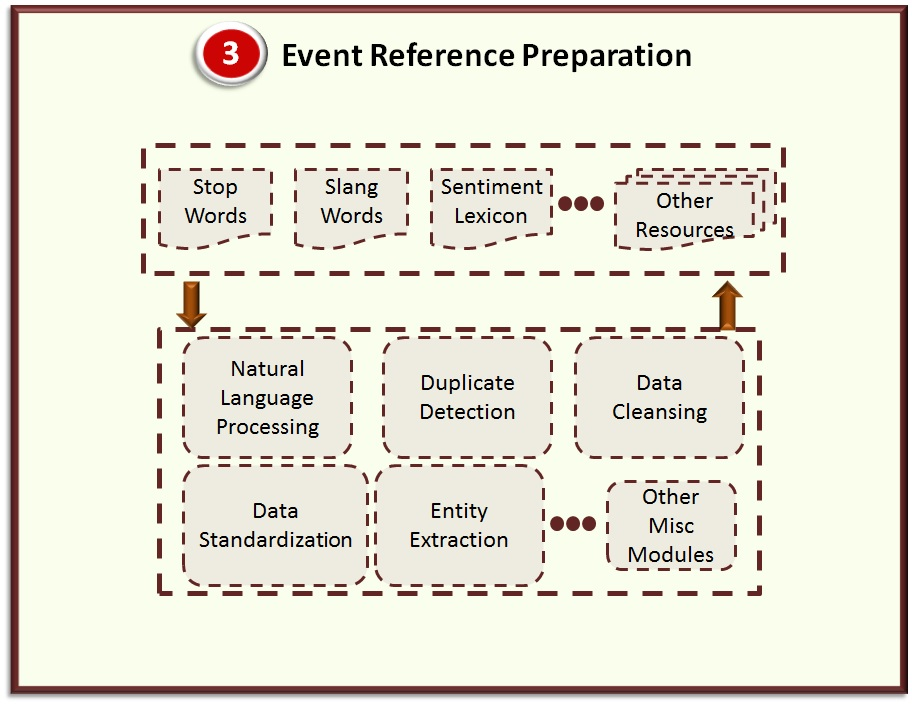
\includegraphics[width=14cm,height=11cm]{Figures/EIIMComponents/EventReferencePreparation.jpg}
\end{figure}

Preprocessing the raw references is an important stage of any data intensive application. This component performs a series of data preparation steps on the collected event references in order to make them suitable for further processing by the other components of the EIIM life cycle. Several resources are compiled in order to tackle the challenges posed by short informal text prevalent in social media. 

%\subsection{Microblog Reference Preparation}

The tweets collected using the previous component goes through the following pre-processing steps:


\subsection{Parts-of-speech tagging} 
The Natural Language Toolkit (http://nltk.org) POS tagger is used for tagging the raw text of the tweets. All the words of a tweet is assigned one of the following parts-of-speech:
\begin{itemize}
\item Noun
\item Adjective
\item Verb
\item Adverb
\item Preposition
\item Interjection
\item Pronoun
\item Article
\end{itemize}

The tagged tweet is also separately stored and maintained. These tags are used later in different components down the pipeline. The Penn Treebank tags\footnote{https://www.ling.upenn.edu/courses/Fall\_2003/ling001/penn\_treebank\_pos.html} are used for tagging and is parsed accordingly for identifying words with a certain parts-of-speech.

\subsection{Special Character Detection}
All the special characters that are not alphanumeric are detected and the total number of special characters in a tweet is stored.


\subsection{Data Cleansing}
The raw text of the tweet is extracted and cleaned. All the user mentions, hashtags, retweet symbols, URLs and special characters are removed and the entire tweet is converted into lowercase. 

\subsection{Duplicate Detection}
The tweets after cleaning are assigned a md5 hash code, which helps in detecting duplicate content. Tweets having the same hash code are considered to be redundant copies of each other, and only a single copy of the tweet is finally stored in the database. This technique also helps in detecting the retweets of a tweet that contain the same content. Also there are certain tweets that are shared with the same content but has different user mentions and with different combination of the words expressing the content. For example, the following tweets talks about the same video shared by mashable and does not present any new information. 

\begin{itemize}
\item RT @mashable: Timelapse video reveals massive size of New York City protests http://t.co/zhqHpkDLk1 \#MillionsMarchNYC http://t.co/WktxssAfDp
\item RT @dianebhartford: ``@mashable: Timelapse video reveals massive size of New York City protests http://t.co/CE0VIyHnLe \#MillionsMarchNYC htt…
\end{itemize}


After the data cleansing step, the duplicate detection scheme identifies both the tweets to be same and only maintain a single copy. This process occurs in real-time. Whenever, a new tweet is obtained from the straming API, the md5 hashcode is calculated after going through the previous data pre-processing steps. A hashtable is maintained in the memory that is constantly searched for the presence of the generated hashcode. If the hashcode is already present then the tweet is dropped and not stored.

\subsection{Stop Word Detection and Elimination}
A list of English stop words is compiled that is publicly shared in the following URL :  
\begin{itemize}
\item https://github.com/dxmahata/EIIMFramework/blob/master/CodeBase/\\EventIdentityInformationManagement/Resources/englishStopwords.txt
\end{itemize}
This list is used for detecting the stop words in English language tweets. The stop words are eliminated and the number of stop words detected is recorded.

\subsection{Slang Word Detection}
Slang words commonly used on the Internet and twitter specific slang publicly shared by FBI\footnote{https://www.documentcloud.org/documents/1199460-responsive-documents.html\#document/p1} is combined together for compiling a list of English slang words. This list is used for detecting and extracting the slang words from the tweets. The number of slang words detected is recorded. This list is also used later to detect the slang hashtags and slang text units.

The compiled list of twitter specific slang words is publicly shared and can be obtained from the following URL : 
\begin{itemize}
\item https://github.com/dxmahata/EIIMFramework/blob/master/CodeBase/\\EventIdentityInformationManagement/Resources/slangWords.txt
\end{itemize}

\subsection{Feeling Word Detection} 
A list of words expressing feelings on the Internet, obtained from wefeelfine.org is used for detecting and extracting the feeling words from a tweet. The number of feeling words detected is recorded and the extracted feeling words are stored. This list is also publicly available and can be obtained from the following URL :
\begin{itemize}
\item https://github.com/dxmahata/EIIMFramework/blob/master/CodeBase/\\EventIdentityInformationManagement/Resources/feelingWords.txt
\end{itemize}

\subsection{Tokenization}
The tweet obtained after performing the data cleansing steps and elimination of stop words are tokenized into unigram and bigram tokens using the tokenizer module available in NLTK. The set of tokens thus obtained are stored separately.

\subsection{Stemming}
The unigram tokens obtained after tokenization are stemmed and a separate list of stemmed tokens are stored. A standard Porter stemmer available with NLTK library is used for the purpose.


\subsection{Tweet Meta-data Extraction}
Several meta-data that are associated with each tweet obtained from the JSON response of the streaming API are extracted.  Some of these meta-data are :
\begin{itemize}
\item Expanded URLs  
\item Hashtags 
\item Retweet Counts 
\item Favorite Counts
\item User Mentions
\item User Follower Counts
\item Verification Information
\item Time Information 
\end{itemize}

\subsection{Named Entity Extraction}
Named entities such as name of persons, animals, places, cars and organizations are extracted from the raw tweets. For this purpose the entity extraction service of AlchemyAPI\footnote{http://alchemyapi.com} is used. 



%It performs deduplication of tweets using md5 hashing scheme. Redundant copies of a tweet are filtered out keeping a single copy in the database. Parts-of-speech tagging is done using the default POS tagger available in the NLTK  module. A standard list of English stop words is used for eliminating the stop words from the tweet text. All the characters of a tweet are converted into lower case and special characters are removed. The tweets are tokenized into unigram tokens. User mentions, retweet symbol and URLs are removed during tokenization and are not considered as tokens.
%
%A list of words expressing feelings in the internet, obtained from wefeelfine.org is used for detecting and extracting the feeling words from a tweet. Slang words commonly used in the internet and twitter specific slang publicly shared by FBI  is combined together for compiling a list of English slang words. The modules use this list for detecting and extracting the slang words from the tweets, hashtags and text units. Retweet counts, favorite counts, verification information, user follower count, time information and expanded form of the URLs shared in the tweets are extracted from the metadata associated with each tweet, as retrieved using the Twitter API. 


\section{Event Information Quality\label{eventinfoquality}}

\begin{figure}[htbp]
  \caption{Event Information Quality component of the EIIM life cycle.}
  \centering
    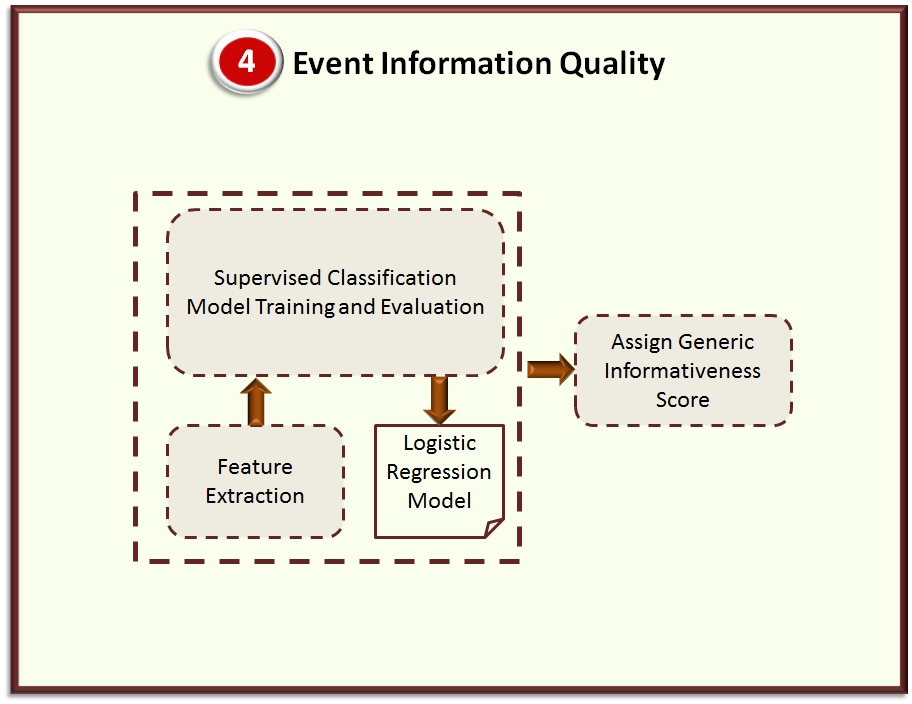
\includegraphics[width=14cm,height=11cm]{Figures/EIIMComponents/EventInformationQuality.jpg}
\end{figure}

This component examines the quality of information present in the tweets collected for the events. It segregates the references having high likelihood of containing good quality event related information from the ones that are less likely to contain or point to good quality information. In order to make a generic module for identifying high quality event related informative references we implemented a logistic regression classifier. Once the classifier is trained, it is used for assigning generic informativeness score to the tweets in real-time as they are collected using the streaming API. The component aids in solving the problem of information overload. Just like an user searching for relevant informative content about an event faces the challenging situation of information overload as discussed in Chapter \ref{challenges}, Section \ref{informationoverload}, it is also a challenge for automated systems to process the huge amount of content coming at high velocity and extract useful information out of it. By filtering out the tweets that are less likely to contain useful and high quality  information it solves the problem of information overload for the other components of the EIIM framework. 

\subsection{Annotated Dataset}
We use a publicly available annotated dataset from the CrisisLex\footnote{http://crisislex.org/data-collections.html} website shared by Olteanu et al. \cite{olteanu2014crisislex}. The collection includes tweets collected during 26 large crisis events in 2012 and 2013, with about 1,000 tweets labeled per crisis for informativeness (i.e. ``informative", or ``not informative"), information type, and source. 28,000 tweets (about 1,000 in each collection) were labeled by crowdsourced workers according to informativeness (informative or not informative), information types (e.g. caution and advice, infrastructure damage), and information sources (e.g. governments, NGOs).

For example, for the Colorado wildfire\footnote{http://en.wikipedia.org/wiki/2012\_Colorado\_wildfires} event, the following tweets were assigned labels of ``related and informative", ``related but not informative", and ``not related", respectively.

\begin{itemize}
\item \textit{Related and Informative} - \#Media Large wildfire in N. Colorado prompts evacuations: Crews are battling a fast-moving wildfire http://t.co/ju1BGTKH \#Politics \#News

\item \textit{Related but not Informative} - RT @LarimerSheriff: \#HighParkFire update \\ http://t.co/hBy5shen

\item \textit{Not Related} - \#Intern \#US \#TATTOO \#Wisconsin \#Ohio \#NC \#PA \#Florida \#Colorado \#Iowa \#Nevada \#Virginia \#NV \#mlb Travel Destinations ; \\ http://t.co/TIHBJKF2
\end{itemize}

Not all the tweets were in English language. We selected English language tweets for training the logistic regression model. There were only 9729 tweets. 

\subsection{Feature Selection and Training}
In order to train the model we assigned a score of 1 to the tweets that were labeled ‘related and informative’, and all the other tweets labeled as ‘related-but not informative’, and ‘not related’ were assigned a score of 0. The choice of features was governed by previous works related to identifying high quality information from Twitter \cite{castillo2011information,gupta2012credibility,vosecky2012searching,huang2011quality}. The list of features selected for the model are: 
\begin{enumerate}
\item \textbf{Has URL} - has a value of 1 if the tweet contains URL or else has a value of 0.
\item \textbf{Number of Words} - total number of unigram tokens extracted from the raw tweet text.
\item \textbf{Number of Stop Words} - total number of English stop words detected in the raw tweet.
\item \textbf{Number of Feeling Words} - total number of feeling words detected in the raw tweet.
\item \textbf{Number of Slang Words} - total number of slang words detected in the raw tweet.
\item \textbf{Number of Hashtags} - total number of hashtags used in the raw tweet.
\item \textbf{Number of User Mentions} - total number of user mentions detected in the raw tweet.
\item \textbf{Tweet Length} - total number of characters used in the raw tweet.
\item \textbf{Unique Characters} - total number of unique characters used in the raw tweet.
\item \textbf{Special Characters} - total number of special characters detected in the tweet.
\item \textbf{Favorite Count} - total number of favorite count of the tweet at the time it was collected.
\item \textbf{Retweet Count} - total number of retweet count of the tweet at the time it was collected.
\item \textbf{Verified} - has a value of 1 if the user posting the tweet is a verified user by Twitter or else has a value of 0.
\item \textbf{Number of Nouns} - total number of nouns detected in the tweet, without considering the hashtags and the user mentions whenever they are tagged as nouns.
\item \textbf{Number of Adjectives} - total number of adjectives detected in the tweet, without considering the hashtags and the user mentions whenever they are tagged as adjectives.
\item \textbf{Number of Verbs} - total number of verbs detected in the tweet, without considering the hashtags and the user mentions whenever they are tagged as verbs.
\item \textbf{Number of Adverbs} - total number of adverbs detected in the tweet, without considering the hashtags and the user mentions whenever they are tagged as adverbs.
\item \textbf{Number of Pronouns} - total number of pronouns detected in the tweet, without considering the hashtags and the user mentions whenever they are tagged as pronouns.
\item \textbf{Number of Interjections} - total number of interjections detected in the tweet, without considering the hashtags and the user mentions whenever they are tagged as interjections.
\item \textbf{Number of Articles} - total number of articles detected in the tweet, without considering the hashtags and the user mentions whenever they are tagged as articles.
\item \textbf{Number of Prepositions} - total number of prepositions detected in the tweet, without considering the hashtags and the user mentions whenever they are tagged as prepositions.
\item \textbf{Formality} - which is defined as follows,
Formality = (\#nouns + \#adjectives + \#prepositions + \#articles - \#pronouns - \#verbs - \#adverbs - \#interjections + 100)/2
and is proposed in \cite{alejandro2011use}. \#nouns, denotes the number of nouns detected in the tweet, and so on.

\end{enumerate}


\begin{table}[htbp]
\centering
\caption{Evaluation measures for logistic regression model.}
\label{logregreseval}
\begin{tabular}{c|c|c|c|}
\cline{2-4}
\multicolumn{1}{l|}{}                          & \textbf{Precision} & \textbf{Recall}       & \textbf{F1-score}     \\ \hline
\multicolumn{1}{|c|}{\textbf{Non-informative} (0)} & 0.70               & 0.49                  & 0.57                  \\ \hline
\multicolumn{1}{|c|}{\textbf{Informative} (1)}     & 0.78               & 0.90                  & 0.84                  \\ \hline
\multicolumn{1}{|c|}{\textbf{Avg/Total}}       & 0.76               & 0.77                  & 0.75                  \\ \hline
\multicolumn{1}{|c}{\textbf{Accuracy}} =  & \multicolumn{1}{l}{} 76.64\%            & \multicolumn{1}{l}{} & \multicolumn{1}{l|}{} \\ \hline
\end{tabular}
\end{table}


\subsection{Model Evaluation}

10-fold cross validation was performed, with `l1' penalty, resulting in a model with an accuracy of 76.64\%. Table \ref{logregreseval} lists the evaluation measures obtained while training the classifier. The ROC AUC Score of the classifier is 0.6934.

\subsection{Assignment of Generic Informativeness Score}
The trained model is used for assigning a score between 0 (least informative) and 1 (most informative) to the tweets in real-time. Both the ‘Event Reference Preparation’ and the ‘Event Information Quality’ components work in collaboration with the ‘Event Reference Collection’ component in order to collect, prepare, assign quality score and store the tweets related to an event, obtained from Twitter streaming API, in real-time.



%\begin{savenotes}
%\begin{table}[ht]
%\centering
%\caption{Tweet features for content informativeness.}
%\label{tweetfeature}
%\begin{tabular}{|l|}
%\hline
%Has Url, No. of words, No. of stopwords, No. of feeling words, No. of slang \\ 
%words, No. of hashtags, No. of user mentions, Tweet  length (No. of characters),\\  No. of unique 
%characters, No. of special characters, Favorite count, Retweet \\ count, Formality, Is tweet verified, No. of nouns, No. of adjectives, No. of \\ verbs, No. of adverbs, No. of pronouns, No. of interjections, No. of articles, \\ No. of prepositions.
% \\ \hline
%\end{tabular}
%\end{table}
%\end{savenotes}



%\subsection{Analysis of Informative and Non-informative Content in Twitter}

\section{Event Identity Information Capture\label{infocapture}}

\begin{figure}[htbp]
  \caption{Event Identity Information Capture component of the EIIM life cycle.}
  \centering
    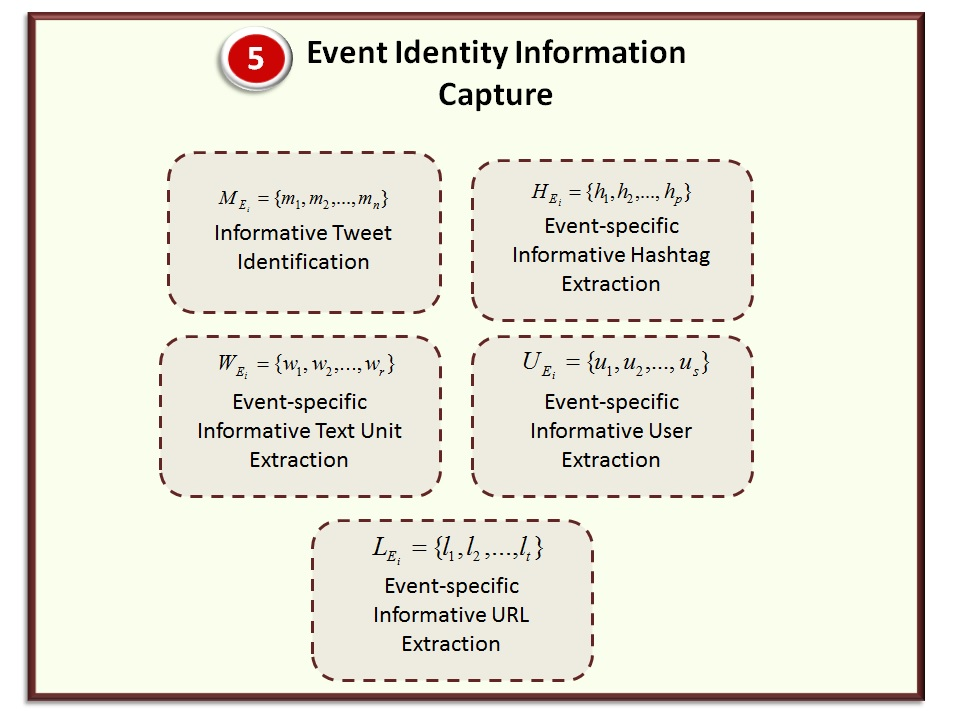
\includegraphics[width=14cm,height=11cm]{Figures/EIIMComponents/EventIdentityInformationCapture.jpg}
\end{figure}

The main functions of this component are:
\begin{itemize}
\item This component aids in extracting event identity information units (explained later) from the already processed tweets and build the Event Identity Information Structure (EIIS) for an event.
\item It enables the framework to set a threshold between 0.0-1.0 for differentiating between high quality informative tweets from low quality non-informative ones related to an event. The event identity information units are then extracted from the high quality informative tweets.
\end{itemize}
  
In order to understand what might consist of the event identity information units that would represent the EIIS, we conducted a detailed analysis of 3.8 million tweets collected for following three events. 
\begin{itemize}
\item CPAC 2014.
\item SXSW 2014.
\item Sochi Winter Games 2014.
\end{itemize}
The analysis and the conclusions we made from it, is presented next.

\subsection{Content Analysis of Event Related Tweets}
Details of the data collected for the analysis are provided in Table \ref{informationcuedata}. The data collection task was accomplished by `Event Reference Collection' component and was then preprocessed by the `Event Reference Preparation' component.

Twitter allows its users to post short messages with a limitation of 140 characters. Users not only post plain textual content in their messages but also share URLs, linking to other external websites, images and videos. The images and videos are 
labeled as media elements by Twitter. Apart from curating new content, the users also share content produced by others. This activity is known as \textit{retweeting}, and such tweets are preceded by the special characters \textit{RT}.
The messages are normally written by a single person and are read by many. The readers in the context of Twitter are known as \textit{followers}, and the user whom the other users follow is considered as their \textit{friend}. Any user with good intent either share messages 
that might be of interest to his followers, or for joining conversations on topics of his interest. The `@' symbol followed by the username commonly known as \textit{user mentions}, is used for mentioning other users in tweets for initiating conversation with them. 

The concise and informal content of a tweet is often contextualized by the use of a crowdsourced annotation scheme called \textit{hashtags}. Hashtags are a sequence of characters in any language prefixed by the symbol `\#' (for e.g. \#icwsm2015). They are widely used
by the users in order to add context to the tweets, categorizing the content based on a topic, join conversations related to a topic, and to make the tweets easily searchable by other interested users. They also act as strong identifiers of topics \cite{laniado2010making}. When tweeting about real-life
events the users also tend to use hashtags in order to post event-specific content. For example `\#Egypt' and `\#Jan25', were among the most popular hashtags in Twitter used for spreading, organizing and analyzing information related to `Egyptian Revolution of 2011' \cite{barrons2012suleiman}. 

Given the mechanisms of user interactions and content production in Twitter, we started our analysis with the assumption that the content of a tweet is primarily composed of hashtags, words for expressing and conveying information, and URLs that lead to additional information about the content. We plotted the distribution of occurrences of all the hashtags, tokens and shared URLs for each event. Due to the short length of the tweets we only considered unigram tokens. We also plotted the distribution of the number of tweets posted by the users.
We observed a power law distribution for all of them (refer Figures \ref{hashtagdist}, \ref{tokendist}, \ref{urldist} and \ref{userdist}). This gave us an intuition that there are skewed sets of hashtags and tokens that are widely used for posting content related to an event. 
%We call them \textit{event-specific hashtags} and \textit{event-specific text units}. 
There is also a specific set of URLs that become popular in comparison to others and a set of users who are more active than others in posting event related content. 

\begin{figure}[htbp]
  \caption{Distribution of hashtags in event related tweets.}
	\label{hashtagdist}
  \centering
    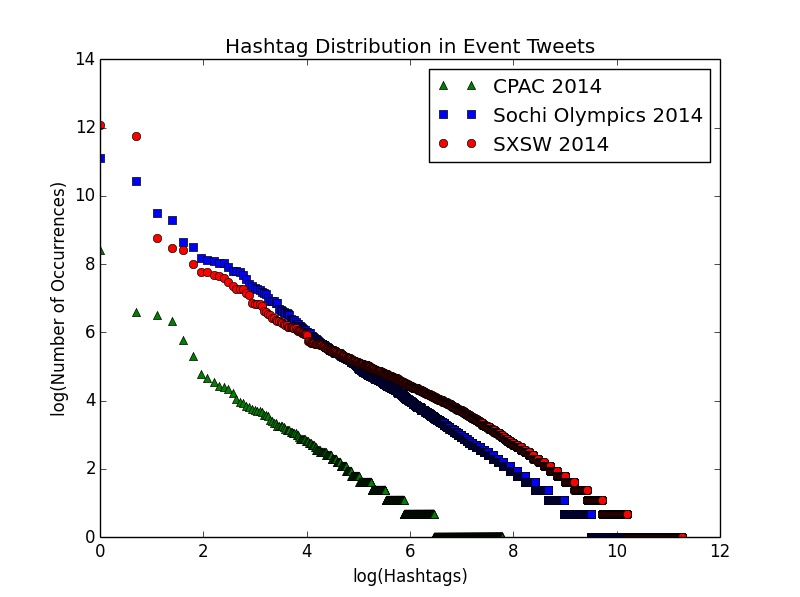
\includegraphics[width=14cm,height=11cm]{Figures/HashTagDistribution.jpeg}
\end{figure}

\begin{figure}[htbp]
  \caption{Distribution of tokens in event related tweets.}
\label{tokendist}
  \centering
    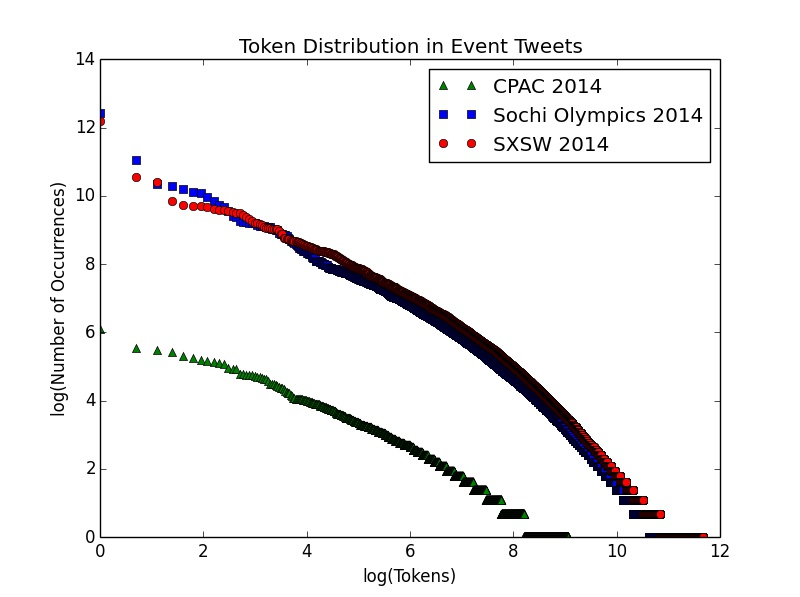
\includegraphics[width=14cm,height=11cm]{Figures/TokenDistribution.jpeg}
\end{figure}

\begin{figure}[htbp]
  \caption{Distribution of URLs in event related tweets.}
\label{urldist}
  \centering
    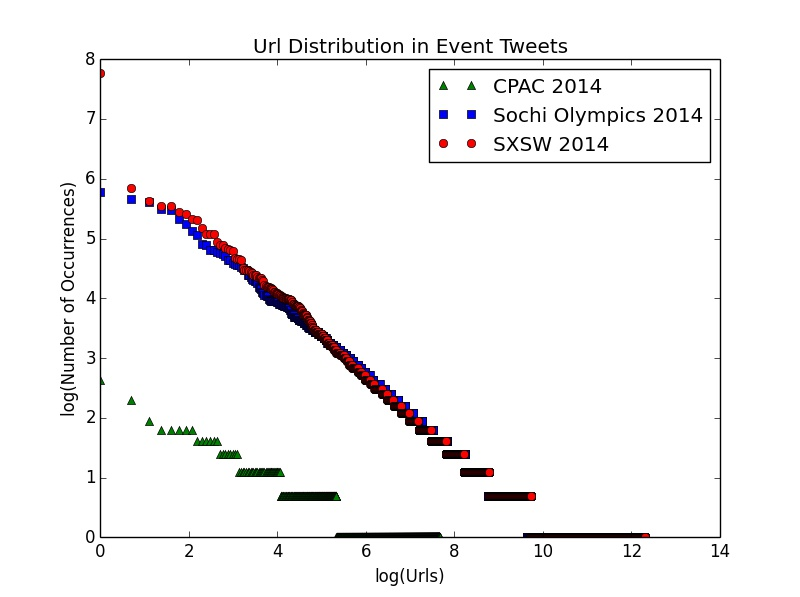
\includegraphics[width=14cm,height=11cm]{Figures/UrlDistribution.jpeg}
\end{figure}

\begin{figure}[htbp]
  \caption{Distribution of users in event related tweets.}
\label{userdist}
  \centering
    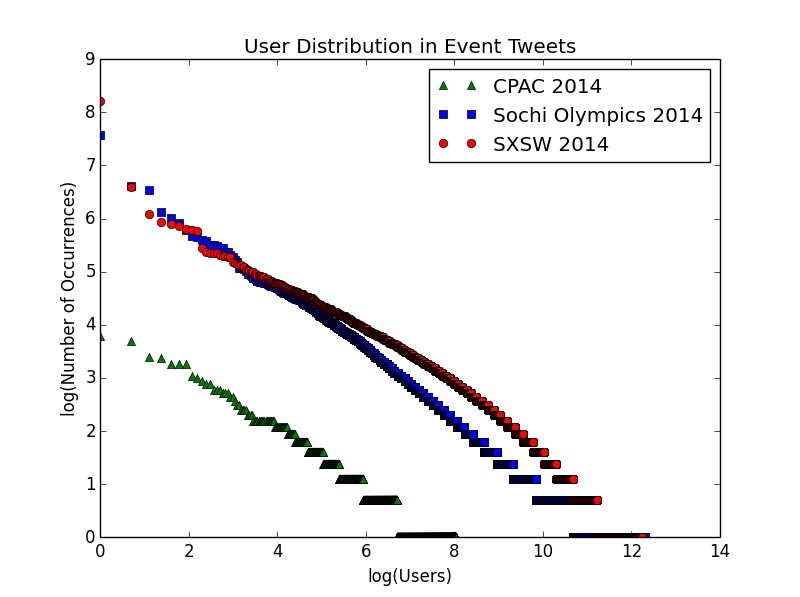
\includegraphics[width=14cm,height=11cm]{Figures/UserDistribution.jpeg}
\end{figure}



Our second step was to use the logistic regression model developed for the `Event Information Quality' component and assign informativeness scores to all the 3.8 million tweets in the dataset. The tweets getting a score greater than 0.7 were considered as instances of high quality informative tweets. Those getting a score lesser than 0.3 were considered as instances of low quality non-informative tweets. We calculated the average values of different content characteristics of the tweets. Top ten percent of the frequently occurring hashtags and nouns were considered as top hashtags and top nouns respectively, for the analysis. Some of the characteristics that were prominently different for informative and non-informative tweets are listed in Table \ref{infoanalysis}.

\begin{figure}[htbp]
\centering
\caption{Content characteristics of informative and non-informative tweets related to events.}
    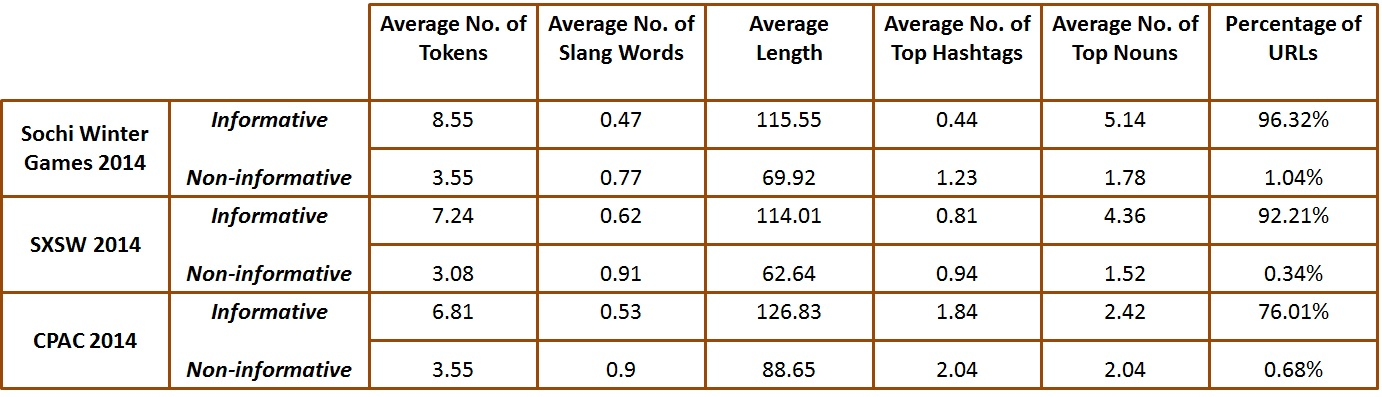
\includegraphics[width=15cm,height=5cm]{Figures/InformationAnalysisTable.jpg}
    
    \label{infoanalysis}
\end{figure}

As presented in the table, some of the observations for all the three events are, 

\begin{itemize}
\item On an average the informative tweets are marked by a higher number of tokens per tweet and greater occurrence of top nouns. 
\item The average length of informative tweets is also more than the non-informative ones. 
\item The percentage of informative tweets having URLs is strikingly high. 
\item A greater use of slang words is observed in non-informative tweets. 
\item Greater occurrence of top hashtags in non-informative tweets intrigued us to look into the content and obtain a detailed view of it. We observed that a lot of non-informative tweets have used popular hashtags with unrelated content and URLs directing to irrelevant information. This is typical of spam tweets as already pointed out in Chapter \ref{challenges}, Section \ref{veracity}. 
\item The average number of follower counts for users posting informative tweets was also observed to be higher than the ones posting non-informative ones. 
\item The average number of feeling words used in informative tweets were also relatively higher than the feeling words used in the non-informative tweets. 
\end{itemize}

The above observations gave us an idea of how high quality informative content related to events is produced in Twitter and the characteristics that differentiate them from low quality non-informative content. We made the following conclusions based on the observations:
\begin{itemize}
\item It is now intuitive that the informative tweets are more expressive, formal and lengthier, marked by higher presence of nouns. 
\item The high presence of nouns indicates that these tweets also contain information about people, places, organizations, etc, associated with the events, which is vital information about any event and is ideal for representing its identity. 
\item Due to the limitations imposed by Twitter on the number of characters in a tweet, the users tend to share URLs along with the textual content that might lead to more information about the event. 
\item Also, users with high follower counts tend to post informative tweets. This can also be concluded by the fact that as they have more followers they are encouraged to share informative content. Conversely, since they share informative content they are followed by a large number of other users interested in the content shared by them.
\end{itemize}

\subsection{Event Identity Information Units}
After the observations in the previous section we conclude that the informative tweets in general are characterized by wordiness, occurrences of URLs and are posted by users with high follower count. These characteristics are also the primary features that distinguish informative from non-informative content. Although, presence of hashtags is not a good indicator of informativeness, yet it is a strong identifier of a topic as already pointed by \cite{laniado2010making}. Popular hashtags for an event might be used maliciously. On the other hand, the presence of a popular hashtag in a wordy tweet consisting of words popular for the event, along with a popular URL, posted by an influential user is highly likely to contain event-specific content. Therefore, it is intuitive that given a stream of tweets for an event an optimal combination of event related popular text units (words, unigrams, bigrams etc),  hashtags, and URLs, posted by an influential user in a tweet, is one of the key indicators for identifying event-specific informative content. It would be highly unlikely for a tweet to contain all of these and yet not convey useful event-specific information. Based on the above analysis we decided to build the EIIS for an event $E_{i}$, composed of the following event identity information units:

\begin{enumerate}
\item A set of tweets $M_{E_{i}} = {\{m_{1_{E_{i}}},m_{2_{E_{i}}}, ... ,m_{n_{E_{i}}}\}}$, related to the event $E_{i}$, having high chances of containing informative content.
\item A set of hashtags $H_{E_{i}} = \{h_{1_{E_{i}}},h_{2_{E_{i}}},..., h_{p_{E_{i}}} \}$, used for annotating the tweets ($\in M_{E_{i}}$) related to event $E_{i}$.
\item A set of text units $W_{E_{i}} = \{w_{1_{E_{i}}},w_{2_{E_{i}}},..., w_{r_{E_{i}}} \}$, used for expressing textual content in tweets ($\in M_{E_{i}}$), related to event $E_{i}$.
\item A set of URLs $L_{E_{i}} = \{l_{1_{E_{i}}},l_{2_{E_{i}}},..., l_{t_{E_{i}}} \}$, shared in the tweets ($\in M_{E_{i}}$) related to event $E_{i}$.
\item A set of users $U_{E_{i}} = \{u_{1_{E_{i}}},u_{2_{E_{i}}},..., u_{s_{E_{i}}} \}$, tweeting the tweets ($\in M_{E_{i}}$), about the event $E_{i}$.
\end{enumerate}

\subsection{Extracting Event Identity Information Units}
The event identity information units for an event $E_{i}$, as defined above are extracted from the event dataset. Following steps are taken:
\begin{itemize}
\item A threshold for the informativeness score assigned in the previous component is set between 0.0-1.0, for extracting the tweets ($\in M_{E_{i}}$). We set a threshold of 0.7. Therefore, the tweets having an informativeness score greater than or equal to 0.7 are filtered out and comprises the set $M_{E_{i}}$.
\item The hashtags that were extracted in the `Event Reference Preparation' step from the tweets $\in M_{E_{i}}$, are used for populating the set $H_{E_{i}}$. However, the hashtags that matches the slang words and stop words are not considered. This is done in order to ensure good quality of information contextualized by the hashtags.
\item The nouns that were extracted in the `Event Reference Preparation' step from the tweets $\in M_{E_{i}}$, are considered as the text units ($\in W_{E_{i}}$). The nouns that matches the slang words are not considered. This is done in order to ensure good quality of textual content represented by the nouns. In another experiment, we considered the extracted named entities as the text units. We report our results and compare the results obtained in both the cases in the next Chapter.
\item The expanded URLs from the meta-data of the tweets $\in M_{E_{i}}$ populates the set $L_{E_{i}}$.
\item The meta-information of the users posting the tweets $\in M_{E_{i}}$, represented by their user ids, is extracted for populating the set $U_{E_{i}}$ 
\end{itemize}  

These event identity information units forms the Event Identity Information Structure (EIIS), as explained next.

\section{Event Identity Information Structure (EIIS)}
This is the component that maintains a persistent EIIS as introduced in Chapter \ref{events}, Section \ref{problem}, for each individual event tracked by the framework and updates the metadata of the EIIS throughout the EIIM life cycle. Due to the unstructured nature of the social media references and evolving nature of the events, we store the event identity information units extracted by the previous component along with their associated meta-data, in a persistent graph data structure stored in the database. We update the meta-data related to each node of the graph using the normal database updation queries. Adjacency lists are used for representing the graph. The choice of storing the event identity information units in a graph structure is also motivated by the wide array of graph processing algorithms used for natural language processing and text mining operations. We show the efficacy and the advantages of a graph in the next section. 

\begin{itemize}
\item Therefore the EIIS is a graph $\mathbf{G_{E_{i}} = (V_{E_{i}},D_{E_{i}})}$, where $\mathbf{V_{E_{i}} = M_{E_{i}} \cup H_{E_{i}} \cup W_{E_{i}} \cup U_{E_{i}} \cup}$ \\  $\mathbf{L_{E_{i}}}$, is the set of vertices and $\mathbf{D_{E_{i}}}$ is the set of directed edges between different vertices. Whenever two vertices are associated, there are two edges between them that are oppositely directed. For example, if a tweets consist of hashtags, text units, URLs and is posted by an user, then there are bi-directed edges between each one of them. 
\end{itemize}




\begin{figure}[htbp]
  \caption{Event Identity Information Structure component of the EIIM life cycle.}
  \centering
    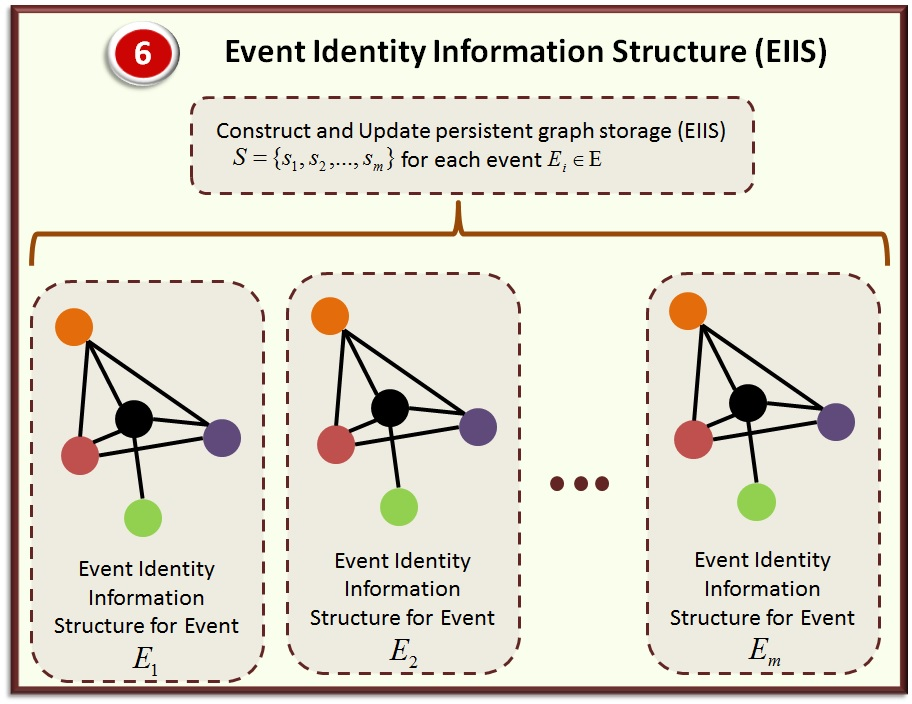
\includegraphics[width=14cm,height=11cm]{Figures/EIIMComponents/EventIdentityInformationStructure.jpg}
\end{figure}


\begin{figure}[htbp]
  \caption{Event Identity Information Processing component of the EIIM life cycle.}
  \centering
    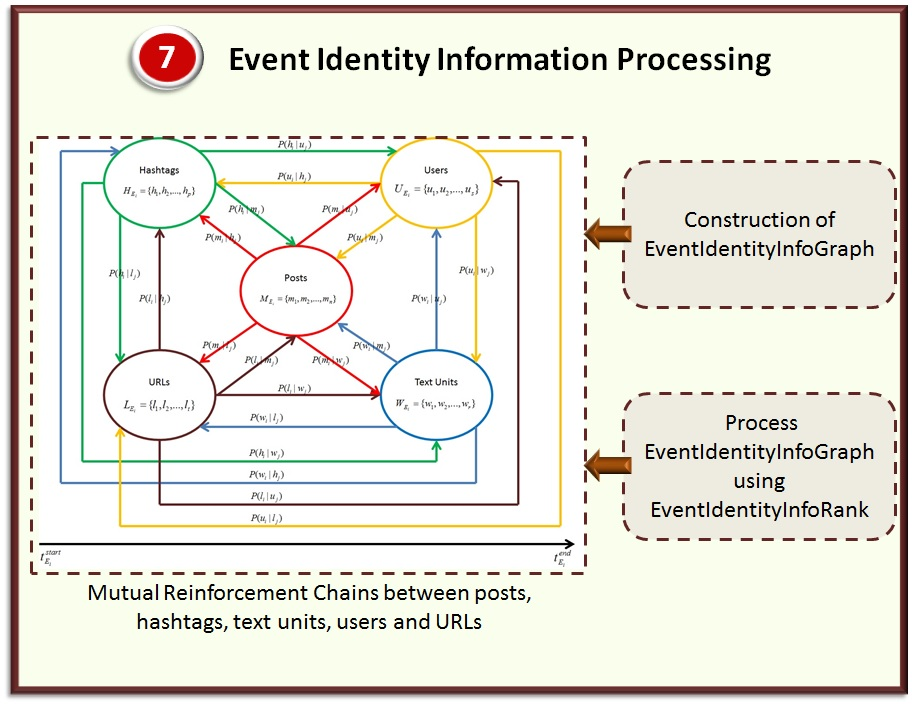
\includegraphics[width=14cm,height=11cm]{Figures/EIIMComponents/EventIdentityInformationProcessing.jpg}
\end{figure}

\section{Event Identity Information Processing\label{EventIdentityInformationProcessing}}
This is the most important processing component of the EIIM life cycle and is at the heart of the entire framework. We make our most novel contributions in this component. The component is mainly divided into two sub-components:
\begin{itemize}
\item \textbf{EventIdentityInfoGraph} - that represents and defines novel relationships between the vertices of the graph $\mathbf{G}$ representing the EIIS.
\item \textbf{EventIdentityInfoProcess} - processes the \textit{EventIdentityInfoGraph} in order to rank its nodes and identify the top most informative event identity information units that acts as inputs to the next two components of the EIIM life cycle.
\end{itemize}

\subsection{EventIdentityInfoGraph\label{eventidentityinfograph}}

We implement a novel graph structure - \textit{EventIdentityInfoGraph}, which is dynamically generated from the graph $\mathbf{G}$ (EIIS), after a configurable interval of time, using following assumptions.
  
For an event $E_{i}$ 
\begin{itemize} 
\item a \textit{tweet is an event-specific informative tweet} if it is strongly associated with:
\begin{itemize}
\item[\textbf{(a)}] \textit{event-specific informative hashtags}, 
\item[\textbf{(b)}] \textit{event-specific informative text units}, 
\item[\textbf{(c)}] \textit{event-specific informative users},
\item[\textbf{(d)}] \textit{event-specific informative URLs}. 
\end{itemize}
\end{itemize}

\begin{itemize} 
\item a \textit{hashtag is an event-specific informative hashtag} if it is strongly associated with:
\begin{itemize}
\item[\textbf{(a)}] \textit{event-specific informative tweets},
\item[\textbf{(b)}] \textit{event-specific informative text units},
\item[\textbf{(c)}] \textit{event-specific informative users},
\item[\textbf{(d)}] \textit{event-specific informative URLs}.
\end{itemize}
\end{itemize}

\begin{itemize} 
\item a \textit{text unit is an event-specific informative text unit} if it is strongly associated with:
\begin{itemize}
\item[\textbf{(a)}] \textit{event-specific informative tweets}, 
\item[\textbf{(b)}] \textit{event-specific informative hashtags}, 
\item[\textbf{(c)}] \textit{event-specific informative users}, 
\item[\textbf{(d)}] \textit{event-specific informative URLs}. 
\end{itemize}
\end{itemize}

\begin{itemize} 
\item a \textit{user is an event-specific informative user} if it is strongly associated with:
\begin{itemize}
\item[\textbf{(a)}] \textit{event-specific informative tweets}, 
\item[\textbf{(b)}] \textit{event-specific informative hashtags}, 
\item[\textbf{(c)}] \textit{event-specific informative text units},
\item[\textbf{(d)}] \textit{event-specific informative URLs}. 
\end{itemize}
\end{itemize}

\begin{itemize} \item a \textit{URL is an event-specific informative URL} if it is strongly associated with:
\begin{itemize}
\item[\textbf{(a)}] \textit{event-specific informative tweets}, 
\item[\textbf{(b)}] \textit{event-specific informative hashtags}, 
\item[\textbf{(c)}] \textit{event-specific informative text units},
\item[\textbf{(d)}] \textit{event-specific informative users}. 
\end{itemize}
\end{itemize}

%\end{itemize}

The relationships for an event $E_{i}$ as stated above, forms a \textit{Mutual Reinforcement Chain} \cite{wei2008query} for the event $E_{i}$ as shown in Figure \ref{mrc}. We represent this relationship in a graph $\mathbf{G_{E_{i}(t)} = (V_{E_{i}(t)},D_{E_{i}(t)})}$, which we call as \textit{EventIdentityInfoGraph}, where $V_{E_{i}(t)} = M_{E_{i}} \cup H_{E_{i}} \cup W_{E_{i}} \cup U_{E_{i}} \cup L_{E_{i}}$, is the set of vertices and $\mathbf{D_{E_{i}(t)}}$ is the set of directed edges between different vertices. The graph $G_{E_{i}(t)}$ is basically, a snapshot of the EIIS structure of the event $E_{i}$ at time t. 

\begin{figure}[htbp]
\centering
\caption{\small Mutual Reinforcement Chains in Twitter for an event.}    
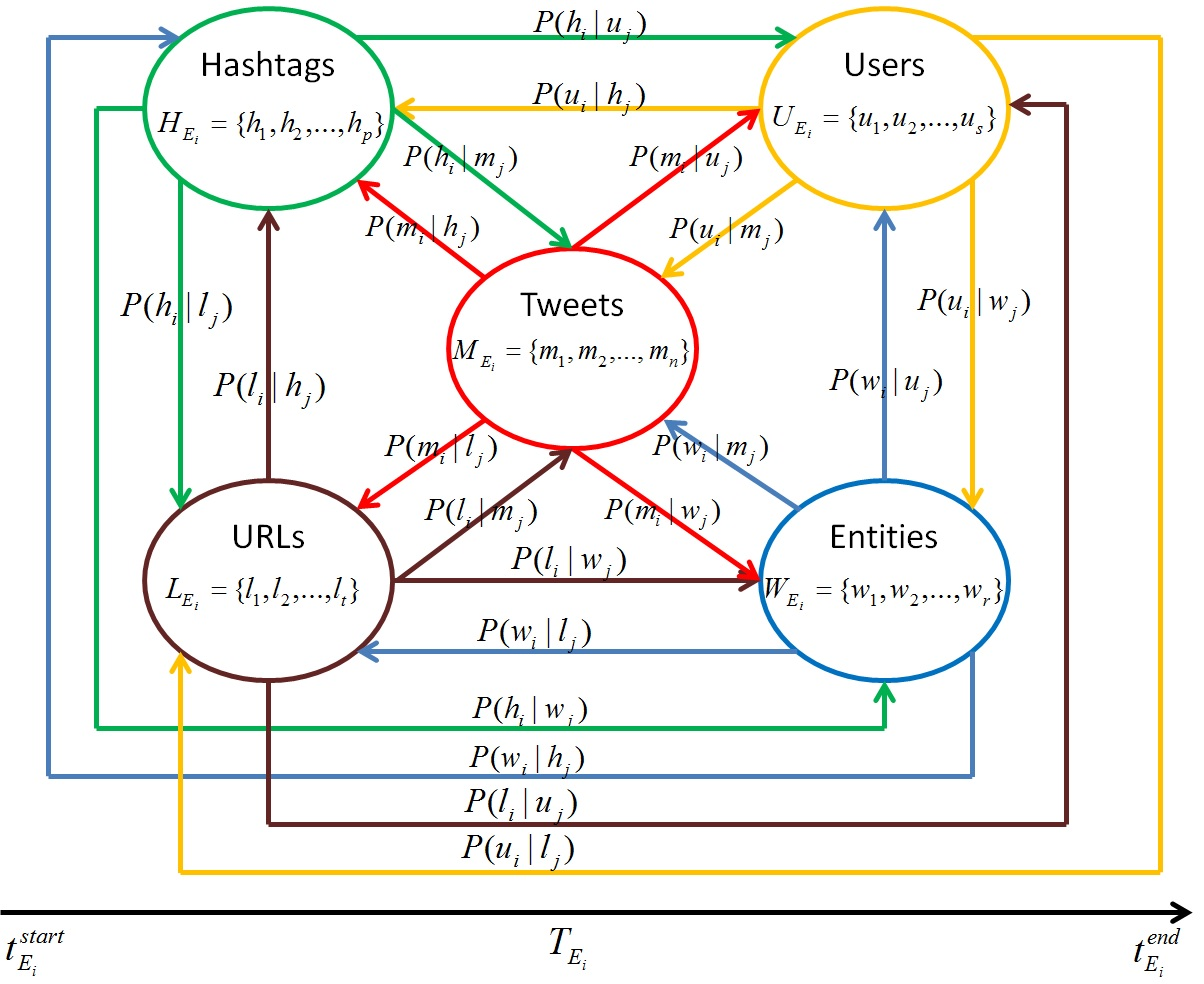
\includegraphics[width=16cm,height=12cm]{Figures/TwitterEventInfoGraph.jpg}
\label{mrc}
\end{figure}
 

Whenever two vertices are associated, there are two edges between them that are oppositely directed. Each directed edge is assigned a weight, which determines the degree of association of one vertex with the other. The weights for each edge is calculated according to the conditional probabilities as given by equations 5.1-5.18. 

\begin{equation}
P(h_{i_{E_{i}}} \mid w_{j_{E_{i}}}) = \frac{No. \, of \, tweets \, h_{i_{E_{i}}} \, and \, w_{j_{E_{i}}} \, occur \, together}{No. \, of \, tweets \, w_{j_{E_{i}}} \, occurs}
\end{equation}

\begin{equation}
P(w_{i_{E_{i}}} \mid h_{j_{E_{i}}}) = \frac{No. \, of \, tweets \, w_{i_{E_{i}}} \, and \, h_{j_{E_{i}}} \, occur \, together}{No. \, of \, tweets \, h_{j_{E_{i}}} \, occurs}
\end{equation}

\begin{equation}
P(h_{i_{E_{i}}} \mid l_{j_{E_{i}}}) = \frac{No. \, of \, tweets \, h_{i_{E_{i}}} \, and \, l_{j_{E_{i}}} \, occur \, together}{No. \, of \, tweets \, l_{j_{E_{i}}} \, occurs}
\end{equation}

\begin{equation}
P(l_{i_{E_{i}}} \mid h_{j_{E_{i}}}) = \frac{No. \, of \, tweets \, l_{i_{E_{i}}} \, and \, h_{j_{E_{i}}} \, occur \, together}{No. \, of \, tweets  \, h_{j_{E_{i}}} \, occurs}
\end{equation}

\begin{equation}
P(h_{i_{E_{i}}} \mid u_{j_{E_{i}}}) = \frac{No. \, of \, tweets  \, h_{i_{E_{i}}} \, and \, u_{j_{E_{i}}} \, occur \, together}{No. \, of \, tweets  \, u_{j_{E_{i}}} \, occurs}
\end{equation}

\begin{equation}
P(u_{i_{E_{i}}} \mid h_{j_{E_{i}}}) = \frac{No. \, of \, tweets  \, u_{i_{E_{i}}} \, and \, h_{j_{E_{i}}} \, occur \, together}{No. \, of \, tweets  \, h_{j_{E_{i}}} \, occurs}
\end{equation}

\begin{equation}
P(w_{i_{E_{i}}} \mid l_{j_{E_{i}}}) = \frac{No. \, of \, tweets  \, w_{i_{E_{i}}} \, and \, l_{j_{E_{i}}} \, occur \, together}{No. \, of \, tweets  \, l_{j_{E_{i}}} \, occurs}
\end{equation}

\begin{equation}
(l_{i_{E_{i}}} \mid w_{j_{E_{i}}}) = \frac{No. \, of \, tweets  \, l_{i_{E_{i}}} \, and \, w_{j_{E_{i}}} \, occur \, together}{No. \, of \, tweets  \, w_{j_{E_{i}}} \, occurs}
\end{equation}

\begin{equation}
P(u_{i_{E_{i}}} \mid l_{j_{E_{i}}}) = \frac{No. \, of \, tweets  \, u_{i_{E_{i}}} \, and \, l_{j_{E_{i}}} \, occur \, together}{No. \, of \, tweets  \, l_{j_{E_{i}}} \, occurs}
\end{equation}

\begin{equation}
P(l_{i_{E_{i}}} \mid u_{j_{E_{i}}}) = \frac{No. \, of \, tweets  \, l_{i_{E_{i}}} \, and \, u_{j_{E_{i}}} \, occur \, together}{No. \, of \, tweets  \, u_{j_{E_{i}}} \, occurs}
\end{equation}

\begin{equation}
P(h_{i_{E_{i}}} \mid m_{j_{E_{i}}}) = 1.0
\end{equation}

\begin{equation}
P(m_{i_{E_{i}}} \mid h_{j_{E_{i}}}) = 1.0
\end{equation}

\begin{equation}
P(w_{i_{E_{i}}} \mid m_{j_{E_{i}}}) = 1.0
\end{equation}

\begin{equation}
P(m_{i_{E_{i}}} \mid w_{j_{E_{i}}}) = 1.0
\end{equation}

\begin{equation}
P(u_{i_{E_{i}}} \mid m_{j_{E_{i}}}) = 1.0
\end{equation}

\begin{equation}
P(m_{i_{E_{i}}} \mid u_{j_{E_{i}}}) = 1.0
\end{equation}

\begin{equation}
P(l_{i_{E_{i}}} \mid m_{j_{E_{i}}}) = 1.0
\end{equation}

\begin{equation}
P(m_{i_{E_{i}}} \mid l_{j_{E_{i}}}) = 1.0
\end{equation}


We do not consider an edge between two vertices of same type. That is, we don't connect a tweet with another tweet. Similarly, for hashtags, text units, users and URLs. This constraint was imposed in order to deal with the nepotistic relationships between high quality content and low quality content introduced by the malicious users for promoting the low quality content as explained in Chapter \ref{challenges}, Section \ref{veracity}.  



%\begin{table*}[ht]
%\caption{Affinity scores of edges between vertices of TwitterEventInfoGraph}
%\label{edgescores}
%\begin{tabular}{|l|}
%\hline 
%\underline{\textbf{\textit{Affinity scores (edge weights) between different vertices}} $\in M_{E_{i}}, H_{E_{i}}, W_{E_{i}}, U_{E_{i}},$} \\ \underline{\textbf{\textit{$L_{E_{i}}$:}}} \\ \\
%$P(h_{i} \mid w_{j}) = \frac{No. \, of \, tweets \, h_{i} \, and \, w_{j} \, occur \, together}{No. \, of \, tweets \, w_{j} \, occurs}$, $P(w_{i} \mid h_{j}) = \frac{No. \, of \, tweets \, w_{i} \, and \, h_{j} \, occur \, together}{No. \, of \, tweets \, h_{j} \, occurs}$, \\
%
%
%$P(h_{i} \mid l_{j}) = \frac{No. \, of \, tweets \, h_{i} \, and \, l_{j} \, occur \, together}{No. \, of \, tweets \, l_{j} \, occurs}$,
%$P(l_{i} \mid h_{j}) = \frac{No. \, of \, tweets \, l_{i} \, and \, h_{j} \, occur \, together}{No. \, of \, tweets  \, h_{j} \, occurs}$, \\
%
%$P(h_{i} \mid u_{j}) = \frac{No. \, of \, tweets  \, h_{i} \, and \, u_{j} \, occur \, together}{No. \, of \, tweets  \, u_{j} \, occurs}$,
%$P(u_{i} \mid h_{j}) = \frac{No. \, of \, tweets  \, u_{i} \, and \, h_{j} \, occur \, together}{No. \, of \, tweets  \, h_{j} \, occurs}$,  \\
%
%$P(w_{i} \mid l_{j}) = \frac{No. \, of \, tweets  \, w_{i} \, and \, l_{j} \, occur \, together}{No. \, of \, tweets  \, l_{j} \, occurs}$, 
%$P(l_{i} \mid w_{j}) = \frac{No. \, of \, tweets  \, l_{i} \, and \, w_{j} \, occur \, together}{No. \, of \, tweets  \, w_{j} \, occurs}$, \\ 
%
%$P(w_{i} \mid u_{j}) = \frac{No. \, of \, tweets  \, w_{i} \, and \, u_{j} \, occur \, together}{No. \, of \, tweets  \, u_{j} \, occurs}$,
%$P(u_{i} \mid w_{j}) = \frac{No. \, of \, tweets  \, u_{i} \, and \, w_{j} \, occur \, together}{No. \, of \, tweets  \, w_{j} \, occurs}$, \\
%
%$P(u_{i} \mid l_{j}) = \frac{No. \, of \, tweets  \, u_{i} \, and \, l_{j} \, occur \, together}{No. \, of \, tweets  \, l_{j} \, occurs}$, 
%$P(l_{i} \mid u_{j}) = \frac{No. \, of \, tweets  \, l_{i} \, and \, u_{j} \, occur \, together}{No. \, of \, tweets  \, u_{j} \, occurs}$, \\
%
%
%$P(h_{i} \mid m_{j}) = P(m_{i} \mid h_{j}) = P(w_{i} \mid m_{j}) = P(m_{i} \mid w_{j}) = P(u_{i} \mid m_{j}) = P(m_{i} \mid u_{j}) =$ \\ $P(l_{i} \mid m_{j})= P(m_{i} \mid l_{j})= 1.0$  \\ \\ 
%\textbf{Note:} $P(h_{i} \mid w_{j})$ should be read as the probability of occurrence of hashtag $h_{i}$ given \\ the occurrence of the text unit $w_{j}$ in the stream of  tweets $M_{E_{i}}$ related to event $E_{i}$ \\ collected over the time period $T_{E_{i}}$. Similarly, for others.\\
%\hline 
%\end{tabular}
%\end{table*}










Next, we explain \textit{EventIdentityInfoRank}.

%%%%%%%%%%%%%%%%%%%%%%%%%%%%%%%%%%%%%%%%%%%%%%%%%%%%%%%%%%%%%%%%%%%%%%%%%%%%%%%%%%
%%%%%%%%%%%%%%%%%                                       TwitterEventInfoRank Subsection                    %%%%%%%%%%%%%%%%%%%%%%%%%%%%%%%%%%
%%%%%%%%%%%%%%%%%%%%%%%%%%%%%%%%%%%%%%%%%%%%%%%%%%%%%%%%%%%%%%%%%%%%%%%%%%%%%%%%%%

\subsection{EventIdentityInfoRank\label{eventidentityinforank}}
\textit{EventIdentityInfoRank} is an iterative algorithm that takes into account the mutually reinforcing relationships between the vertices of \textit{EventIdentityInfoGraph} as explained in the previous section and propagates event-specific scores of each vertex to connected vertices across the graph for ranking its vertices ($\in V_{E_{i}(t)}$) in terms of event-specific informativeness.

We first assign a event-specific score to all the vertices of the graph. Event-specific scores for vertices $(\in H_{E_{i}}, W_{E_{i}}, U_{E_{i}}, L_{E_{i}})$ are calculated using equations 5.19-5.22. The tweets  $(\in M_{E_{i}})$ are assigned an initial informativeness score as obtained from the logistic regression model in `Event Information Quality' component. The event-specific scores for vertices $(\in H_{E_{i}}, W_{E_{i}}, U_{E_{i}}, L_{E_{i}})$ and informativeness score for vertices $(\in M_{E_{i}})$ gives an initial ranking of all the vertices of \textit{EventIdentityInfoGraph}. We aim to refine the initial scores and assign a final score for ranking the vertices by leveraging the mutually reinforcing relationships between them.
\begin{equation}
Score(h_{i_{E_{i}}}) = \frac{freq(h_{i})}{max\{freq(h_{1}),freq(h_{2}),...,freq(h_{p})\}}
\end{equation}

\begin{equation}
Score(w_{i_{E_{i}}}) = \frac{freq(w_{i})}{max\{freq(w_{1}),freq(w_{2}),...,freq(w_{r})\}}
\end{equation}

\begin{equation}
Score(u_{i_{E_{i}}}) = \frac{followers(u_{i})}{max\{followers(u_{1}),...,followers(u_{r})\}}
\end{equation}

\begin{equation}
Score(l_{i_{E_{i}}}) = \frac{freq(l_{i})}{max\{freq(l_{1}),freq(l_{2}),...,freq(l_{r})\}}
\end{equation}


The relationships between two different subsets of vertices in graph $\mathbf{G_{E_{i}(t)}}$ is denoted by an affinity matrix. For e.g., $\mathbf{A_{E_{i}}^{MH}}$ denotes the $\mathbf{M_{E_{i}}-H_{E_{i}}}$ affinity matrix for event $E_{i}$, where $\mathbf{(i,j)^{th}}$ entry is the edge weight quantifying the association between $i^{th}$ tweet ($\in M_{E_{i}}$) and $j^{th}$ hashtag ($\in H_{E_{i}}$), calculated using equations 5.1-5.18. Similarly, $\mathbf{A_{E_{i}}^{WH}}$ denotes the $\mathbf{W_{E_{i}}-H_{E_{i}}}$ affinity matrix between set of text units $W_{E_{i}}$ and set of hashtags $H_{E_{i}}$ for event $E_{i}$, and so on.


The rankings of \textit{tweets}, \textit{hashtags}, \textit{text units}, \textit{users} and \textit{URLs} in terms of event-specific informativeness, can be iteratively derived from the Mutual Reinforcement Chain for the event. Let $R_{{E_{i}}}^{M}$, $R_{{E_{i}}}^{H}$, $R_{{E_{i}}}^{W}$, $R_{{E_{i}}}^{U}$ and $R_{{E_{i}}}^{L}$ denote the ranking scores for the set of tweets ($\in M_{E_{}}$), set of  hashtags $(\in H_{E_{i}})$, set of text units $(\in W_{E_{i}})$, set of users $(\in U_{E_{i}})$, and set of URLs $(\in L_{E_{i}})$, respectively. Therefore, the Mutual Reinforcement Chain ranking for the $k^{th}$ iteration can be formulated as follows:
 

%\begin{equation}
%\tiny R_{{E_{i}}}^{M(k+1)} = A_{E_{i}}^{MM(k)}R_{{E_{i}}}^{M(k)} + A_{E_{i}}^{MH(k)}R_{{E_{i}}}^{H(k)} + A_{E_{i}}^{MW(k)}R_{{E_{i}}}^{W(k)} + A_{E_{i}}^{MU(k)}R_{{E_{i}}}^{U(k)} + A_{E_{i}}^{ML(k)}R_{{E_{i}}}^{L(k)}
%\end{equation}

\begin{equation}
R_{{E_{i}}}^{M(k+1)} = A_{E_{i}}^{MM(k)}R_{{E_{i}}}^{M(k)} + A_{E_{i}}^{MH(k)}R_{{E_{i}}}^{H(k)} + A_{E_{i}}^{MW(k)}R_{{E_{i}}}^{W(k)}+ A_{E_{i}}^{MU(k)}R_{{E_{i}}}^{U(k)} + A_{E_{i}}^{ML(k)}R_{{E_{i}}}^{L(k)}
\end{equation}

%\begin{equation}
%\tiny R_{{E_{i}}}^{H(k+1)} = A_{E_{i}}^{HM(k)}R_{{E_{i}}}^{M(k)} + A_{E_{i}}^{HH(k)}R_{{E_{i}}}^{H(k)} + A_{E_{i}}^{HW(k)}R_{{E_{i}}}^{W(k)} + A_{E_{i}}^{HU(k)}R_{{E_{i}}}^{U(k)} + A_{E_{i}}^{HL(k)}R_{{E_{i}}}^{L(k)}
%\end{equation}

\begin{equation}
R_{{E_{i}}}^{H(k+1)} = A_{E_{i}}^{HM(k)}R_{{E_{i}}}^{M(k)} + A_{E_{i}}^{HH(k)}R_{{E_{i}}}^{H(k)} + A_{E_{i}}^{HW(k)}R_{{E_{i}}}^{W(k)}+ A_{E_{i}}^{HU(k)}R_{{E_{i}}}^{U(k)} + A_{E_{i}}^{HL(k)}R_{{E_{i}}}^{L(k)}
\end{equation}



%\begin{equation}
%\tiny R_{{E_{i}}}^{W(k+1)} = A_{E_{i}}^{WM(k)}R_{{E_{i}}}^{M(k)} + A_{E_{i}}^{WH(k)}R_{{E_{i}}}^{H(k)} + A_{E_{i}}^{WW(k)}R_{{E_{i}}}^{W(k)} + A_{E_{i}}^{WU(k)}R_{{E_{i}}}^{U(k)} + A_{E_{i}}^{WL(k)}R_{{E_{i}}}^{L(k)}
%\end{equation}

\begin{equation}
R_{{E_{i}}}^{W(k+1)} = A_{E_{i}}^{WM(k)}R_{{E_{i}}}^{M(k)} + A_{E_{i}}^{WH(k)}R_{{E_{i}}}^{H(k)} + A_{E_{i}}^{WW(k)}R_{{E_{i}}}^{W(k)}+ A_{E_{i}}^{WU(k)}R_{{E_{i}}}^{U(k)} + A_{E_{i}}^{WL(k)}R_{{E_{i}}}^{L(k)}
\end{equation}

%\begin{equation}
%\tiny R_{{E_{i}}}^{U(k+1)} = A_{E_{i}}^{UM(k)}R_{{E_{i}}}^{M(k)} + A_{E_{i}}^{UH(k)}R_{{E_{i}}}^{H(k)} + A_{E_{i}}^{UW(k)}R_{{E_{i}}}^{W(k)} + A_{E_{i}}^{UU(k)}R_{{E_{i}}}^{U(k)} + A_{E_{i}}^{UL(k)}R_{{E_{i}}}^{L(k)}
%\end{equation}

\begin{equation}
R_{{E_{i}}}^{U(k+1)} = A_{E_{i}}^{UM(k)}R_{{E_{i}}}^{M(k)} + A_{E_{i}}^{UH(k)}R_{{E_{i}}}^{H(k)} + A_{E_{i}}^{UW(k)}R_{{E_{i}}}^{W(k)}+ A_{E_{i}}^{UU(k)}R_{{E_{i}}}^{U(k)} + A_{E_{i}}^{UL(k)}R_{{E_{i}}}^{L(k)}
\end{equation}

%\begin{equation}
%\tiny R_{{E_{i}}}^{L(k+1)} = A_{E_{i}}^{LM(k)}R_{{E_{i}}}^{M(k)} + A_{E_{i}}^{LH(k)}R_{{E_{i}}}^{H(k)} + A_{E_{i}}^{LW(k)}R_{{E_{i}}}^{W(k)} + A_{E_{i}}^{LU(k)}R_{{E_{i}}}^{U(k)} + A_{E_{i}}^{LL(k)}R_{{E_{i}}}^{L(k)}
%\end{equation}


\begin{equation}
R_{{E_{i}}}^{L(k+1)} = A_{E_{i}}^{LM(k)}R_{{E_{i}}}^{M(k)} + A_{E_{i}}^{LH(k)}R_{{E_{i}}}^{H(k)} +A_{E_{i}}^{LW(k)}R_{{E_{i}}}^{W(k)}+ A_{E_{i}}^{LU(k)}R_{{E_{i}}}^{U(k)}+ A_{E_{i}}^{LL(k)}R_{{E_{i}}}^{L(k)}
\end{equation}


The equations 5-9 can be represented in the form of a block matrix $\Delta_{E_{i}}$, where,
\[ \Delta_{E_{i}} = \left( \begin{array}{ccccc}
A_{E_{i}}^{MM} & A_{E_{i}}^{MH} & A_{E_{i}}^{MW} &  A_{E_{i}}^{MU} & A_{E_{i}}^{ML} \\
A_{E_{i}}^{HM} & A_{E_{i}}^{HH} & A_{E_{i}}^{HW} & A_{E_{i}}^{HU} & A_{E_{i}}^{HL} \\
A_{E_{i}}^{WM} & A_{E_{i}}^{WH} & A_{E_{i}}^{WW} & A_{E_{i}}^{WU} & A_{E_{i}}^{WL}\\
A_{E_{i}}^{UM} & A_{E_{i}}^{UH} & A_{E_{i}}^{UW} & A_{E_{i}}^{UU} & A_{E_{i}}^{UL} \\
A_{E_{i}}^{LM} & A_{E_{i}}^{LH} & A_{E_{i}}^{LW} & A_{E_{i}}^{LU} & A_{E_{i}}^{LL} \end{array} \right)\] 

Let \[R_{E_{i}} = \left( \begin{array}{c}
R_{{E_{i}}}^{M} \\
R_{{E_{i}}}^{H} \\
R_{{E_{i}}}^{W} \\
R_{{E_{i}}}^{U} \\
R_{{E_{i}}}^{L} \end{array} \right)\] 

then, $R_{E_{i}}$ can be computed as the dominant eigenvector of $\Delta_{E_{i}}$.
\begin{equation}
\Delta_{E_{i}}.R_{E_{i}} = \lambda.R_{E_{i}}
\end{equation}

In order to guarantee a unique $R_{E_{i}}$, $\Delta_{E_{i}}$ must be forced to be stochastic and irreducible. 

To make $\Delta_{E_{i}}$ stochastic we divide the value of each element in a column of $\Delta_{E_{i}}$ by the sum of the values of all the elements in that column. This finally makes $\Delta_{E_{i}}$ column stochastic. We now denote it by $\hat \Delta_{E_{i}}$.
%we remove all the rows and columns of the block matrices whose all elements are zeros. Since, we don't consider edges between two vertices of same type, all the elements of the diagonal block matrices are zero by default. We then 

Next, we make $\hat \Delta_{E_{i}}$ irreducible. This is done by making the graph $G$ strongly connected by adding links from one node to any other node with a probability vector $p$. Now, $\hat \Delta_{E_{i}}$ is transformed to 

\begin{equation}
\overline \Delta_{E_{i}} = \alpha \hat \Delta_{E_{i}} + (1-\alpha)E
\end{equation}
\begin{equation}
E = p \times [1]_{1 \times k}
\end{equation}
where $0 \le \alpha \le 1$ is set to 0.85 according to \textit{PageRank}, and k is the order of $\hat \Delta_{E_{i}}$. We set $p = [1/k]_{k \times 1}$ by assuming a uniform distribution over all elements. Now, $\overline \Delta_{E_{i}}$ is stochastic and irreducible and it can be shown that it is also primitive by checking $\overline \Delta_{E_{i}}^{2}$ is greater than $0$.

Following steps are taken next,
\begin{itemize}
\item[\textbf{1.}] We initialize the rank vectors ($ R_{{E_{i}}}^{M(0)}, R_{{E_{i}}}^{H(0)}, R_{{E_{i}}}^{W(0)}, R_{{E_{i}}}^{U(0)}, R_{{E_{i}}}^{L(0)}$) for each subset of vertices ($M_{E_{i}}, H_{E_{i}}, W_{E_{i}}, U_{E_{i}}, L_{E_{i}}$). We use the event-specific scores calculated for the set of hashtags, text units, users and urls as their initial scores. All the scores lie between 0 and 1. For the tweets we use the logistic regression model and assign each one of them an initial informativeness score between 0 and 1.

\item[\textbf{2.}] Then we assign
\[ R_{E_{i}}^{0} = \left( \begin{array}{c}
R_{{E_{i}}}^{M(0)} \\
R_{{E_{i}}}^{H(0)} \\
R_{{E_{i}}}^{W(0)} \\
R_{{E_{i}}}^{U(0)} \\
R_{{E_{i}}}^{L(0)} \end{array} \right)\] 

and normalize $R_{E_{i}}^{0}$ such that $\mid \mid R_{E_{i}}^{0}\mid \mid_{1} = 1$

\item[\textbf{3.}] Apply power iteration method using the same parameters as used in PageRank with the convergence tolerance set at 1e-08 and $\lambda = 0.85$ .

\item[\textbf{4.}] We get the final rank vectors for each subset of the vertices ($R_{{E_{i}}}^{M}, R_{{E_{i}}}^{H}, R_{{E_{i}}}^{W}, R_{{E_{i}}}^{U}, R_{{E_{i}}}^{L}$) after convergence. 

\item[\textbf{5.}] We finally obtain the subsets $\hat{M}_{E_{i}}, \hat{H}_{E_{i}}, \hat{W}_{E_{i}}, \hat{L}_{E_{i}}, \hat{U}_{E_{i}}$ consisting of the \textit{tweets}, \textit{hashtags}, \textit{text units}, \textit{URLs} and \textit{users}, respectively arranged in descending order of their final scores.

\end{itemize}

The final ordered subsets $\mathbf{\hat{M}_{E_{i}}, \hat{H}_{E_{i}}, \hat{W}_{E_{i}}, \hat{L}_{E_{i}}, \hat{U}_{E_{i}}}$,  thus obtained are the tweets, hashtags, text units, URLs and users, ranked in terms of their event-specific informativeness. The entire procedure is presented step-by-step in an Algorithm \ref{algo}.

\begin{algorithm}
\caption{EventIdentityInfoRank algorithm}
\label{algo}
\SetKwData{Left}{left}\SetKwData{This}{this}\SetKwData{Up}{up}
\SetKwFunction{Union}{Union}\SetKwFunction{FindCompress}{FindCompress}
\SetKwInOut{Input}{Input}\SetKwInOut{Output}{Output}
\Input{Sets of vertices $M_{E_{i}},H_{E_{i}}, W_{E_{i}}, U_{E_{i}}, L_{E_{i}}$ of graph $G_{E_{i}(t)}$, $\alpha=0.85$, $\varepsilon=1e-08$.}
\BlankLine
\Output{Ordered set of vertices $\hat{M}_{E_{i}}$, containing tweets ranked in order of event-specific informative content sharing information about event related entities.}
\BlankLine
\textbf{Steps:}
\BlankLine
Initialize rank vectors $[R_{{E_{i}}}^{M(0)}, R_{{E_{i}}}^{H(0)}, R_{{E_{i}}}^{W(0)}, R_{{E_{i}}}^{U(0)}, R_{{E_{i}}}^{L(0)}]$\;
\BlankLine
Assign $R_{E_{i}}^{0}=[R_{E_{i}}^{M(0)},R_{E_{i}}^{H(0)},R_{E_{i}}^{W(0)},R_{E_{i}}^{U(0)},R_{E_{i}}^{L(0)}]^{T} $\;
\BlankLine
Normalize $R_{E_{i}}^{0}$ such that $\mid \mid R_{E_{i}}^{0}\mid \mid_{1} = 1$ \;
\BlankLine
Construct matrix $\Delta_{E_{i}}$\;
\BlankLine
Make matrix $\Delta_{E_{i}}$ stochastic and irreducible converting it to $\overline \Delta_{E_{i}}$\;
\BlankLine
$k \leftarrow 1$ 
\BlankLine
\Repeat{$\mid \mid R_{E_{i}}^{k} - R_{E_{i}}^{k-1} \mid \mid_{1} < \varepsilon \; OR \; k \ge 100$}{$R_{E_{i}}^{k} \leftarrow \overline \Delta_{E_{i}}R_{E_{i}}^{k-1}$\;
$k \leftarrow k+1$\; }
\BlankLine
$R_{E_{i}}^{M} \leftarrow R_{E_{i}}^{M(k)}$, $R_{E_{i}}^{H} \leftarrow R_{E_{i}}^{H(k)}$, $R_{E_{i}}^{W} \leftarrow R_{E_{i}}^{W(k)}$,  $R_{E_{i}}^{U} \leftarrow R_{E_{i}}^{U(k)}$, $R_{E_{i}}^{L} \leftarrow R_{E_{i}}^{L(k)}$\;
\BlankLine
$\hat{M}_{E_{i}} \leftarrow R_{E_{i}}^{M}$, $\hat{H}_{E_{i}} \leftarrow R_{E_{i}}^{H}$, $\hat{W}_{E_{i}} \leftarrow R_{E_{i}}^{W}$, $\hat{U}_{E_{i}} \leftarrow R_{E_{i}}^{U}$, $\hat{L}_{E_{i}} \leftarrow R_{E_{i}}^{L}$\;
\BlankLine
return $\hat{M}_{E_{i}}$,$\hat{H}_{E_{i}}$,$\hat{W}_{E_{i}}$,$\hat{U}_{E_{i}}$,$\hat{L}_{E_{i}}$\;
%\caption{\scriptsize Algorithm for ranking the nodes of G}\label{algo_disjdecomp}
\end{algorithm}\DecMargin{1em}

%During the implementation of the \textit{TwitterEventInfoRank} algorithm the slang hashtags were removed. We only considered nouns as the text units and removed the slang words. We already reported in our analysis that non-informative tweets have higher slang content. Therefore, removal of slang hashtags and text units was done in order to obtain high quality results. We also showed higher occurrence of nouns in informative tweets. Also, the occurrence of a noun in a tweet intuitively suggests that the tweet has information about a person, place, or thing. Thus, we only considered the set of nouns extracted from the tweets as the set of text units. 

%The text units are generic units in the framework and can be changed according to specific requirements. Entities extracted from the textual content of tweets could be experimented, in place of nouns. 
Since the algorithm uses power iteration method for ranking the vertices of a graph, it could be easily made scalable using mapreduce paradigm \cite{lin2010design}. We plan to work on it in the future and implement our framework using hadoop and mapreduce environment. Also, the EIIM framework takes a hybrid approach by using both supervised and unsupervised component, it is easily applicable in situations where an event needs to be tracked over time. The supervised portion assigns an initial generic informativeness score to the tweets for bootstrapping an unsupervised process that finally assigns event-specific informativeness scores. When applied over a time period the method for assigning the initial supervised scores might remain the same and the unsupervised process can change the rankings of the tweet contents as the event evolves. 


\section{Event Reference Resolution}

\begin{figure}[htbp]
  \caption{Event Reference Resolution component of the EIIM life cycle.}
  \centering
    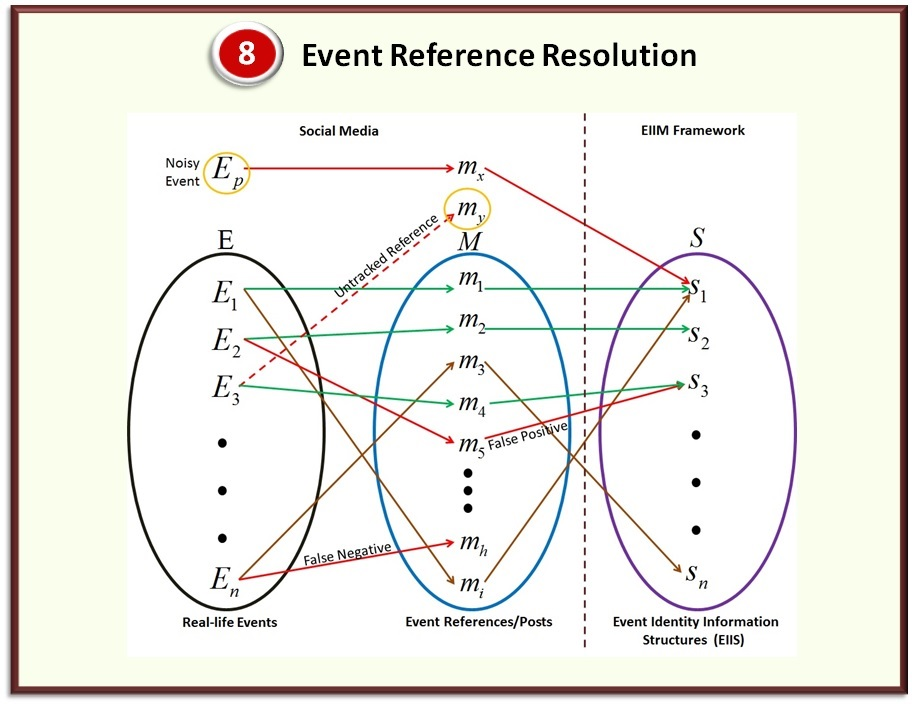
\includegraphics[width=14cm,height=11cm]{Figures/EIIMComponents/EventReferenceResolution.jpg}
\end{figure}

One of the main aims of the EIIM framework is to assign the reference of an event $E_{i}$ to its corresponding Entity Identity Information Structure ($s_{E_{i}}$). This aim is executed by this component. The main functions are as follows:

\begin{itemize}
\item The output of the previous component assigns a final ranked event-specific informativeness scores to the tweets. Using this score the component allows to choose top k tweets ranked in terms of their event-specific informative content. This enable the identification and resolution of high quality tweets providing useful information about the event $E_{i}$, solving the problems of \textit{noisy events} and \textit{noisy references} as already discussed in Chapter \ref{events}, Section \ref{problem}. The tweets after the top K are thrown away from the EIIS. This results in extremely high quality, event-specific informative tweets in the EIIS. We performed our experiment on the two events:

\begin{itemize}
\item Sydney Siege Crisis
\item Millions March NYC
\end{itemize}

Excerpts of the top 5 tweets identified for both the events are given below.

\textbf{Top Five Event-specific Informative Tweet Excerpts for Sydney Siege Event}
\begin{enumerate}
\item RT @faithcnn: Hostage taker in Sydney cafe has demanded 2 things: ISIS flag and; phone call with Australia PM Tony Abbott \#SydneySiege http://t.co/a2vgrn30Xh
\item Aussie grand mufti and; Imam Council condemn \#Sydneysiege hostage capture http://t.co/ED98YKMxqM - LIVE UPDATES http://t.c...
\item RT @PatDollard: \#SydneySiege: Hostages Held By Jihadis In Australian Cafe - WATCH LIVE VIDEO COVERAGE http://t.co/uGxmd7zLpc \#tcot \#pjnet \\ sydney-siege-scene/index.html
\item RT @FoxNews: MORE: Police confirm 3 hostages escape Sydney cafe, unknown number remain inside http://t.co/pcAt91LIdS \#Sydneysiege
\item Watch \#sydneysiege police conference live as hostages are still being held inside a central Sydney cafe http://t.co/OjulBqM7w2 \#c4news
\end{enumerate}

\item The other task that can be achieved using this component is the extraction of extremely informative features from the ranked results of the previous component and use them to form an evolutionary classifier or a feature vector for constantly tracking the event tweets w.r.t time. But the feature may get updated as the event progresses and a new set of ranked features needs to be obtained from the previous component after an interval of time that should be configurable. This, functionality of the component is currently not implemented and tested. We consider it as one of our future works.
\end{itemize}


\section{Event Analytics}
\begin{figure}[htbp]
  \caption{Event Analytics component of the EIIM life cycle.}
  \centering
    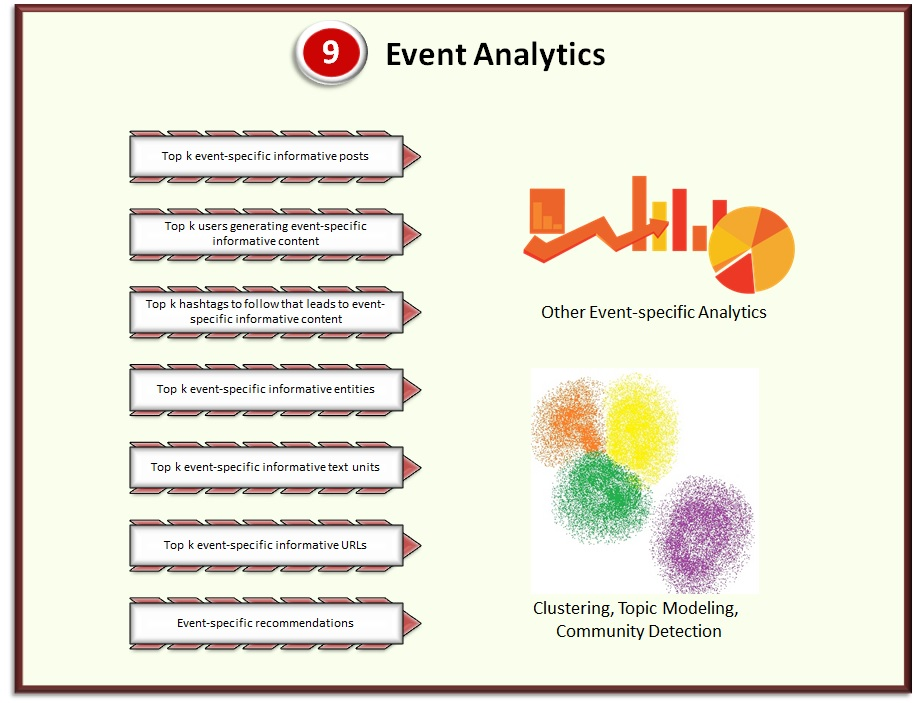
\includegraphics[width=14cm,height=11cm]{Figures/EIIMComponents/EventAnalytics.jpg}
\end{figure}

The outputs of the Event Identity Information Processing component after processing the EventIdentityInfoGraph of a particular event is used for generating different analytics related to the event for the chosen time period, by this component. Some of the immediately available analytics that help in extracting deeper insights from the event related content are shown below for our sample events.

\textbf{Top Five Event-specific Informative Hashtags for Sydney Siege Event}
\begin{enumerate}
\item \#sydneysiege 
\item \#SydneySiege
\item \#Sydneysiege
\item \#MartinPlace
\item \#9News                                                                                                                                                                                                                                                                                                                                                                                                                                                                                                                 
\end{enumerate}

\textbf{Top Five Event-specific Informative Text Units for Sydney Siege Event}
\begin{enumerate}
\item police
\item sydney
\item reporter
\item lindt
\item isis                                                                                                                                                                                                                                                                                                                                                                                                                                                                                                                
\end{enumerate}

\textbf{Top Five Event-specific Informative URLs for Sydney Siege Event}
\begin{enumerate}
\item http://www.cnn.com/2014/12/15/world/asia/australia-sydney-hostage-situation/\\index.html
\item http://www.bbc.co.uk/news/world-australia-30474089
\item http://edition.cnn.com/2014/12/15/world/asia/australia-sydney-siege-scene/\\index.html
\item http://rt.com/news/214399-sydney-hostages-islamists-updates/ 
\item http://www.newsroompost.com/138766/sydney-cafe-siege-ends-gunman-among-two-killed                                                                                                                                                                                                                                                                                                                                                                                                                                                                                                                
\end{enumerate}





\textbf{Three Randomly Selected Tweets for Top Three Event-specific Informative Users posting about Sydney Siege Event.}
\begin{enumerate}
\item \textbf{User 1}
\begin{enumerate}
\item RT @cnni: Hostage taker in Sydney cafe demands ISIS flag and call with Australian PM, Sky News reports. http://t.co/a2vgrn30Xh \#sydneysiege
\item RT @DR\_SHAHID: Hostage taker demands delivery of an \#ISIS flag and a conversation with Prime Minister Tony Abbott http://t.co/xTSDMKCPcD
\item RT @SkyNewsBreak: Update - New South Wales police commissioner confirms five hostages have escaped from the Lindt cafe in Sydney \#sydneysiege
\end{enumerate}

\item \textbf{User 2}
\begin{enumerate}
\item RT @smh: NSW Police Deputy Commissioner Catherine Burn will hold a press conference to update on the \#SydneySiege at 6.30pm.
\item RT @Y7News: Helpful travel advice for commuters heading out of \#Sydney’s CBD this evening - http://t.co/aQx2lvSosm \#sydneysiege
\item RT @hughwhitfeld: British PM David Cameron informed of \#sydneysiege ..UK Foreign Office is in touch with Aus authorities
\end{enumerate}

\item \textbf{User 3}
\begin{enumerate}
\item RT @RT\_com: \#SYDNEY: Gunman tall man in late 40s, dressed in black – eyewitness http://t.co/m51P8dUPhB \#SydneySiege http://t.co/NvJzFsGrFN
\item RT @NewsAustralia: 2GB's Ray Hadley claims hostage takers in \#SydneySiege "wants to speak to Prime Minister Abbott live on radio."
\item RT @BBCWorld: "Profoundly shocking" -Australia PM Tony Abbott delivers second \#sydneysiege statement. MORE: http://t.co/VaKt3ZpRZR
\end{enumerate}

\end{enumerate}

\textbf{Top Five Event-specific Informative Hashtags for Millions March NYC Event}
\begin{enumerate}
\item \#MillionsMarchNYC
\item \#BlackLivesMatter
\item \#ICantBreathe
\item \#ShutItDown
\item \#millionsmarchnyc                                                                                                                                                                                                                                                                                                                                                                                                                                                                                                                 
\end{enumerate}

\textbf{Top Five Event-specific Informative Text Units for Millions March NYC Event}
\begin{enumerate}
\item police
\item nyc
\item eric
\item protesters
\item nypd                                                                                                                                                                                                                                                                                                                                                                                                                                                                                                                
\end{enumerate}

\textbf{Top Five Event-specific Informative URLs for Millions March NYC Event}
\begin{enumerate}
\item http://rt.com/usa/214203-protests-police-brutality-nationwide/\\index.html
\item http://mashable.com/2014/12/13/time-lapse-new-york-protest-march/?utm\_cid=mash-com-Tw-main-link
\item http://www.cbsnews.com/news/eric-garner-ferguson-missouri-protesters-converge-on-washington/
\item http://www.huffingtonpost.com/2014/12/13/millions-march-nyc\_n\_6320348.html?ncid=tweetlnkushpmg00000051 
\item https://www.youtube.com/watch?v=Iz7hkfNmfTY\&feature=youtu.be                                                                                                                                                                                                                                                                                                                                                                                                                                                                                           
\end{enumerate}


\textbf{Three Randomly Selected Tweets for Top Three Event-specific Informative Users posting about Millions March NYC Event for a particular hour.}
\begin{enumerate}
\item \textbf{User 1}
\begin{enumerate}
\item RT @mashable: Timelapse video reveals massive size of New York City protests http://t.co/zhqHpkDLk1 \#MillionsMarchNYC http://t.co/WktxssAfDp
\item RT @DahmPublishing: RT@wendycarrillo: Real thugs wear flag pics and Eric Garner's eyes are haunting image \#MillionsMarchNYC http://t.co/7wY…
\item RT @TheRoot: RT @mfmartinez: Protesters continue gathering in Washington Square Park \#MillionsMarchNYC \#TheRootMOW http://t.co/IwkQG1KjFg
\end{enumerate}

\item \textbf{User 2}
\begin{enumerate}
\item RT @roqchams: Thousands march on NYPD headquarters to protest police terrorism http://t.co/yVyUVYkd9X http://t.co/X4QZrfOISh \#MillionsMarchNYC
\item RT @NYjusticeleague: Hundreds killed. Ten Demands. One Continued Fight.  Sign our petition at: http://t.co/KETNo6bS0V \#MillionsMarchNYC htt…
\item RT @cobismith: Union Square now with NYPD in foreground, \#MillionsMarchNYC protesters at right and; US national debt ticker on the left http:/…
\end{enumerate}

\item \textbf{User 3}
\begin{enumerate}
\item RT @mashable: Timelapse video reveals massive size of New York City protests http://t.co/zhqHpkDLk1 \#MillionsMarchNYC http://t.co/WktxssAfDp
\item RT @KeeganNYC: LOTS of NYPD waiting for protesters on the BK side of the Brooklyn Bridge \#MillionsMarchNYC \#ShutItDown \#ICantBreathe http:/…
\item RT @Zegota42: . @KeeganNYC Protesters on Brooklyn Bridge leaving Manhattan Skyline behind. \#MillionsMarchNYC \#ICantBreathe http://t.co/UPvN…
\end{enumerate}

\end{enumerate}


Some of the other event analytics that can be readily done using the \textit{EventIdentityInfoGraph}, and we would like to explore in the near future are:
\begin{itemize}
\item Topic modeling.
\item Event-specific recommendations.
\item Clustering and Cluster Analysis.
\item Community detection.
\item Trend Analysis.
\end{itemize}

The event related data stored in the database by the `Event Reference Collection' would allow to do all types of analysis that are popular in social media.

